\chapter{软件变更影响域分析}
\label{chap_impact}

本章主要介绍软件变更影响域分析的相关概念、分析方法和工具模块的设计与实现。变更影响域分析主要对补丁引入的变更进行分析并找到其对应的语义影响域,即所谓的变更影响域,以用于后续的冲突检测。

由于软件变更是对程序语法结构所作出的修改,它会将原有的语法结构变更为新的语法结构。因此,考虑到修改前的语法结构与软件中其他语法结构的耦合性,应用软件变更后,这些相关语法结构的行为会受到该软件变更的影响。本文将这些受到补丁中变更影响的语法结构集合称之为变更的语义影响域(即变更影响域)。更详细的定义可以参考章节\ref {sec_impact}。

找到变更的语义影响域需要从代码中挖掘两类信息:
\begin{enumerate}
	\item 代码的变更集合,即两个软件版本之间的语法结构差异性。该集合描述了不同软件版本间的语法结构变更情况。
	\item 变更的影响集合,即受变更集合语义影响的其他程序语法结构。该集合描述了变更所造成的语义影响范围。
\end{enumerate}

上述两类集合可用于确定软件变更对代码的语义影响域。因此,该分析过程可以分为两个步骤。首先,变更影响域分析需要找到不同版本代码之间的软件变更集合。其次,变更影响域分析应根据找到的软件变更集合,分析并得到其变更影响域。可见,变更影响域分析可以拆分为两个相应的子过程,即找到软件变更集合的子过程和获取其变更影响域的子过程。这两个子分析过程可以分别采用程序间语法差异性分析和变更语义影响分析来实现。

因此,该分析方法所对应的影响域分析模块在实现的过程中也应拆分为两个子模块,即差异性分析子模块和影响分析子模块。这两个子模块将分别实现程序间语法差异性分析和变更语义影响分析的过程。由于学术界中已有许多相关的分析算法实现,因此影响域分析模块在实现中将直接将采用已有的分析工具。本文中工具实现的主要精力将放在子模块的整合和调整过程上。

综上所述,软件变更影响域分析的过程也就是找到软件变更,并分析得到变更影响域的过程。这些找到的变更影响域将作为软件变更冲突检测过程中的输入,并用于判断变更影响域之间是否会产生冲突。

下面将分别对这两个子分析过程和其模块设计与实现进行介绍。


%通过语义影响域分析,我们就可以从代码中挖掘出所需要的变更影响域信息,从而可以进行后续的冲突检测工作。
%
%实际上,语义影响域分析主要分为两个子过程,即程序间差异分析和变更语义影响分析,通过这两个分析的协作来完成整个语义影响域的分析。
%
%我们可以将整个语义影响域分析过程定义为如下的函数,该分析过程先将版本演进的过程转化为补丁,再去计算补丁对程序代码的语义影响域:
%
%\begin{definition}
%	$ia: Code \times Code \mapsto {Structure}$。$s = ia(v_i,v_j) = impact(diff(v_i,v_j),v_i),i,j \subset \mathbb{N}$。
%\end{definition}
%
%因此,整个语义影响域分析过程可以用算法\ref {algo_impact}描述。
%
%在兼容性检测工具中,该部分工作被实现为影响域分析模块,该模块需要对$ia$函数进行实际的实现。因此,该模块可以对应地拆分为两个子模块分别进行实现:
%\begin{itemize}
%	\item 差异性分析模块:实现相应的程序差异性分析过程。即$diff$函数的实现。
%	\item 影响分析模块:实现相应的变更语义影响分析过程。即$impact$函数的实现。
%\end{itemize}
%
%该模块中首先需要定义好合适的影响范围和影响元素的级别。
%
%事实上,可以将程序中受变更影响的部分划分为不同的粒度,从而获得不同程度的影响\cite{petrenko2009variable},我们考虑对面向对象的编程方法中的影响元素级别进行划分:
%
%\begin{enumerate}
%	\item 类:探讨变更对于其他类和对象的影响。对于面向对象的程序设计方法而言,这是最高级别的粒度。
%	\item 方法:探讨变更对于其他方法的的影响。
%	\item 基本块:探讨变更对于其他基本块的影响。
%	\item 语句:探讨变更对于其他语句的影响。
%\end{enumerate}
%
%而所谓的影响范围也需要界定其粒度,不同层级的粒度显然会对语义影响域分析的精度产生影响。
%
%\begin{enumerate}
%	\item 类间:考虑变更的影响可能延伸到其他类、对象。
%	\item 方法间:考虑变更的影响可能延伸到其他方法内部。
%	\item 方法内部:考虑变更的影响只在本方法的内部延伸。
%\end{enumerate}
%
%不同级别的影响范围均可分别采用不同的影响元素级别。
%
%在实际情况中,我们主要采用了较为简单的分析过程,即将影响范围限制在方法内部,但是将受影响元素设置为程序语句级别,以保证精度。
%
%在实现该模块的过程中,由于我们可以采用现有工具来完成具体的程序间差异分析和变更语义影响分析过程,因而这两个子过程的分析算法可以直接使用已有的成熟算法。我们可以将主要精力放在如何整合两个子过程,并将其工具实现进行改进,以适用于兼容性检测问题的具体情况。
%
%下面分别对这两个子过程的分析方法和对应模块的设计与实现进行叙述。
%
%\begin{algorithm}[H]
%	\caption{语义影响域分析算法}
%	\label{algo_impact}
%	\begin{algorithmic}[1]
%		\Require $v_i$,$v_j$,即两个不同版本的代码	
%		\Ensure $s$,即版本间的变更对于版本$v_i$的语义影响域
%		\Function {ia}{$v_i,v_j$}
%		\State $p \gets diff(v_i,v_j)$
%		\State $s \gets impact(p,v_i)$
%		\State\Return{$s$}
%		\EndFunction
%	\end{algorithmic}
%\end{algorithm}

\section{程序间语法差异性分析}
\label {chap_diff}

如前所述,程序间语法差异性分析主要是寻找不同版本间的软件变更的过程,该过程需要分析代码间的语法结构差异性,并得到相应的变更集合。该过程主要关注程序间在语法结构上的差异性,最后得到的变更集合也将以语法结构的形式进行描述。


%程序间差异性分析是$diff$函数的实现。它主要用于分析两个不同版本的程序之间的差异性,其结果即我们所需要的程序变更集合。
%
近年来学术界有不少程序间语法差异性分析方面的相关工作,并给出了一些较为成熟的工具实现,因此本文考虑采用已有工具来实现其所对应的差异性分析子模块。

\subsection{相关定义}

本节主要介绍程序间语法差异性分析过程中所涉及到的相关概念和定义,以更清楚的了解该分析过程的实质。

假设$\mathcal{C}$是某个版本的源代码文件中按照该语言的合法语法结构组织起来的代码(如抽象语法树的形式),即由该语言的相应$\mathcal{S}$组成的集合。$\mathcal{S}$是某种语言的合法语法结构,例如Java语言中的语句、方法定义、类定义等,由于随不同语言的实际情况而变化,在这里不做更具体的定义。$v_k$表示第k个版本的代码$\mathcal{C}$,其中$k \subset \mathbb{N}$。

\begin{definition}
	$\mathcal{P}: S \times S$。$\mathcal{P}$是补丁,也就是变更集合,即一个由$\mathcal{S}$的二元组构成的集合。$\forall c \subset \mathcal{P}$,有$c = (s_i,s_j)$,其中$s_i,s_j \subset \mathcal{S},i,j \subset \mathbb{N}$,$s_i$和$s_j$分别表示变更前和变更后的代码语法结构。
\end{definition}

\begin{definition}
	\label {define_diff}
	$diff : \mathcal{C} \times \mathcal{C} \mapsto \mathcal{P}$。该函数用于求解两个不同版本的代码$v_i$和$v_j$之间的语法差异性,其结果即为变更集合$\mathcal{P}$。
\end{definition}

$diff$函数描述了什么是程序间语法差异性分析,它能够接受两个不同版本的代码,并返回代码间的语法结构差异,也就是该分析所要求的变更集合。

\subsection{分析方法}

在本文的兼容性检测方法中,程序间语法差异性分析的主要任务是接受两个不同版本的源代码,并返回代码间的语法结构差异信息。这种结构化的差异信息可以视为补丁的一种,只不过它和常见的采用Unix diff工具生成的纯文本补丁文件相比具有更丰富的信息,能够以该语言的合法语法结构的形式对软件变更进行描述。

根据上一节中的相关定义,该分析过程应该具备如下特征:
\begin{itemize}
	\item 输入为两个不同版本的源代码。即该分析方法应当是针对某种语言的源代码文件进行比对。
	\item 输出为源代码间的软件变更集合。即该分析方法应当找到这些源代码文件之间发生的变更,并以合适的形式将其输出。
	\item 每条变更描述对于该语言的合法语法结构的变更。即该分析方法中所找到的变更应当是该源代码实现语言的合法语法结构之间的变化。
\end{itemize}

除此以外,该分析过程还应当给出更丰富的语法结构信息,以方便后续分析过程的使用,例如:
\begin{itemize}
	\item 每条变更描述变更前后语法结构的相关信息。例如该语法结构的位置信息,该信息能够指示变更的发生位置等,可用于后续分析过程找到该变更对应的代码位置。
	\item 每条变更描述了其所属的作用域,即描述了这些语法结构之间的从属关系。该信息描述了变更的作用范围、所属语法结构等,可用于后续分析过程找到某个限定的作用域范围内作用于某种特定语法结构类型的所有变更。
\end{itemize}

对该分析过程作出这样的要求是为了后续分析过程的方便。由于后续的变更语义影响分析需要我们提供软件变更集合作为输入,而纯文本类型的补丁文件只描述单纯的文本行变更,并不包含语法信息,也就无法从中提取出所需的语法层面的变更信息,因此该类型的程序间文本差异性分析方法是无法满足本文需求的。

在实践过程中,一种比较好的选择是在抽象语法树上进行差异性分析,因为抽象语法树中包括了足够的语法结构信息。

\subsection{模块设计与实现}

本文中的差异性分析模块在实现中采用了jpf-regression自带的前置工具ASTro来进行程序间语法差异性分析过程。该子模块实现了$diff$函数的实际功能,能接受两个不同版本的Java源代码文件作为输入,并以AST的形式输出变更集合。

%\subsubsection{设计}
%
%在该模块的设计中,其输入输出过程可以描述如图\ref {differ},输入输出的具体描述参见表\ref {differ_io}。
%
%\begin{figure}[H]
%	\centering
%	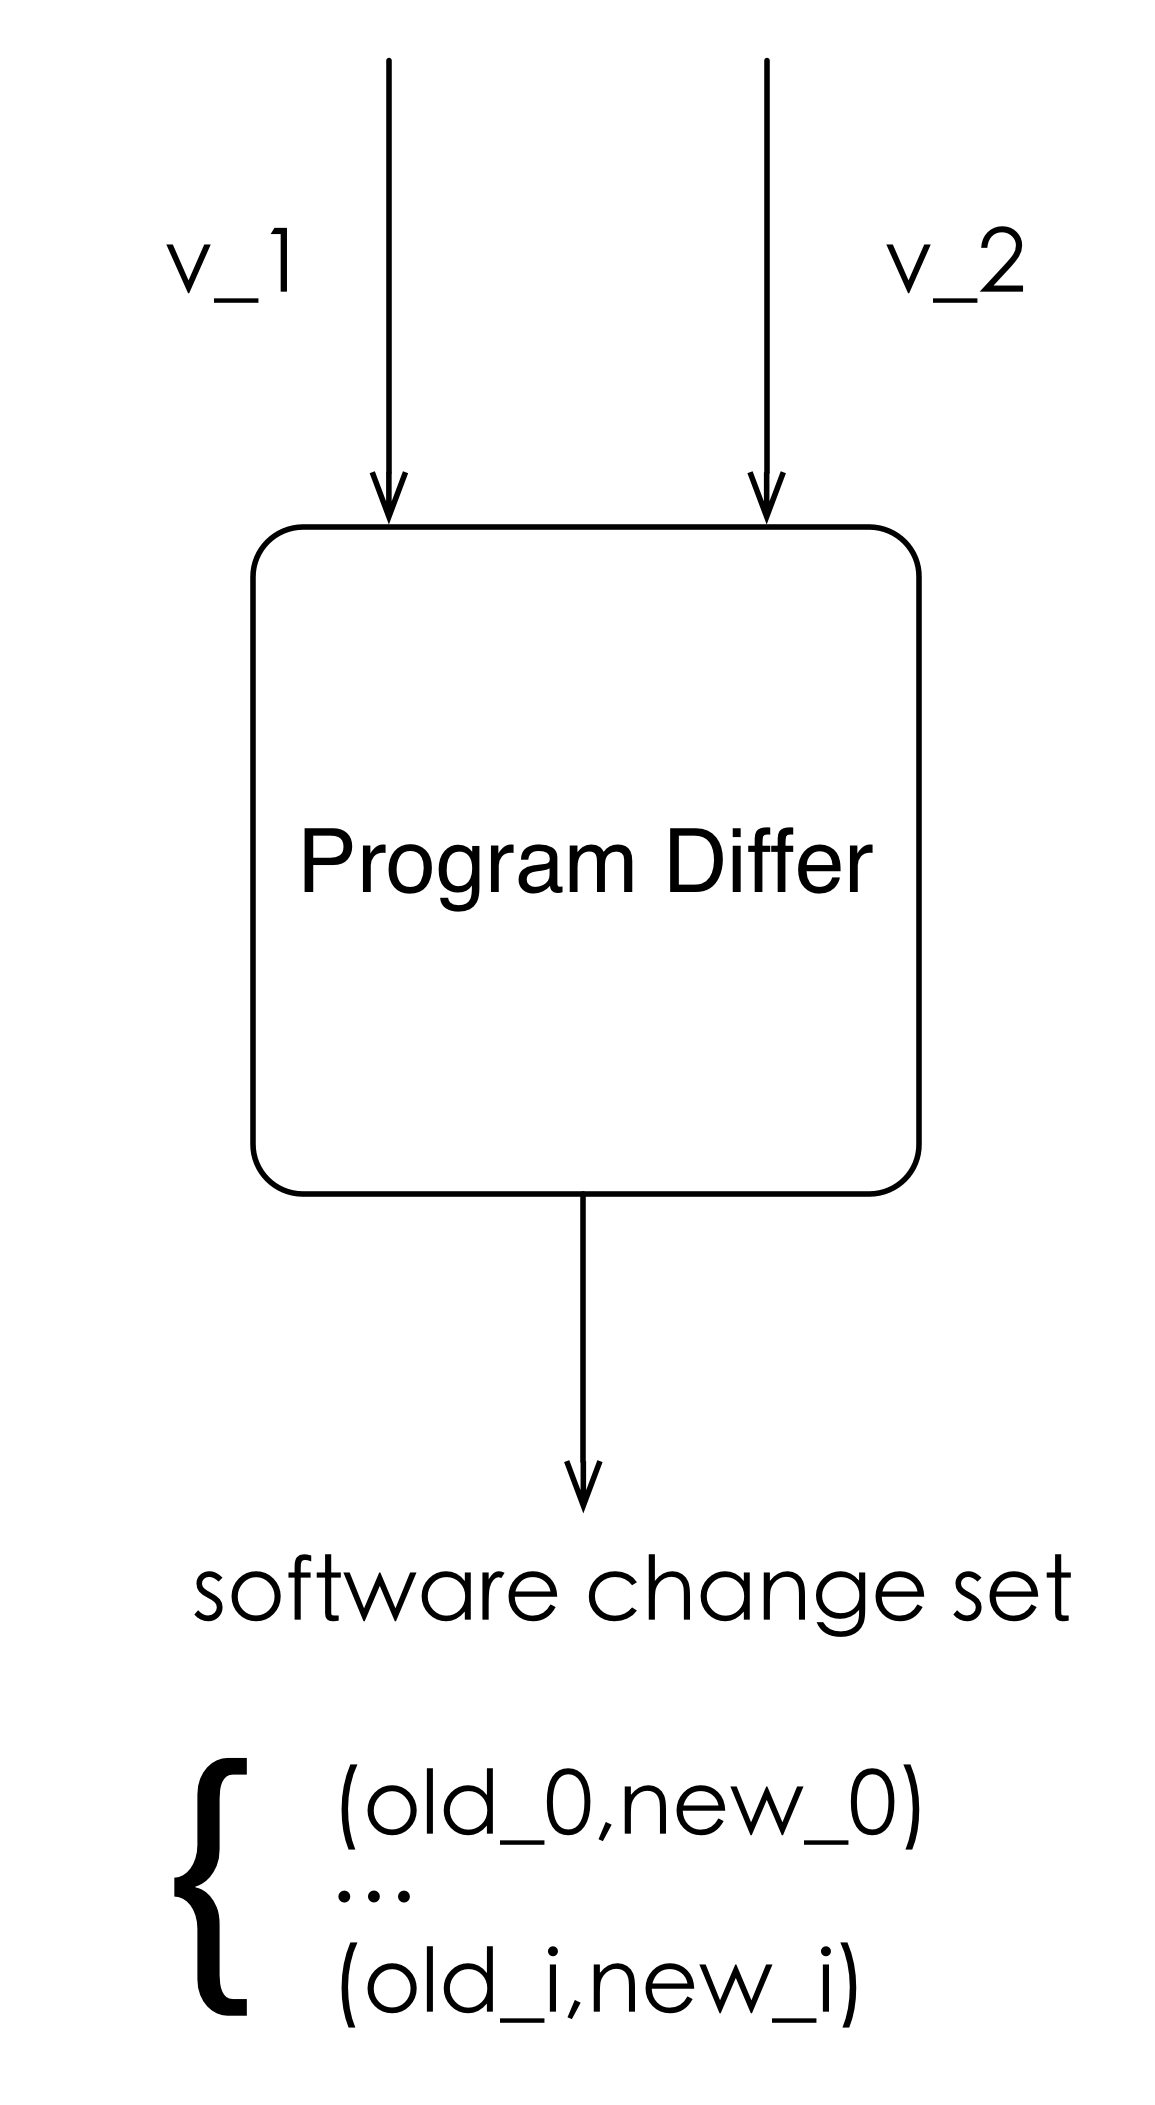
\includegraphics[height=.6\columnwidth]{chap03_differ}
%	\caption {差异性分析模块}
%	\label {differ}	
%\end{figure}
%
%图中所描述的模块输出——软件变更集合,设计为如下的格式,即变更前后的代码结构所组成的二元组集合:
%\begin{definition}
%	$ change\_set = \{ (old_i,new_i) \mid  old_i \subset Structure,new_i \subset Structure, i \subset \mathbb{N} \}$
%\end{definition}
%
%由于该模块需要调用其他工具来完成具体的差异性分析过程,其输出应作为影响分析模块的输入,可见该模块的核心任务包括:
%\begin{itemize}
%	\item 差异性分析
%	\item 输入输出
%\end{itemize}
%
%因此该模块的内部设计可以参考图\ref {des_diff}。
%
%该模块的流程也就可以设计成如下的形式:
%\begin{enumerate}
%	\item 读取输入
%	\item 进行差异性分析
%	\item 输出分析结果
%\end{enumerate}
%
%\begin{figure}[H]
%	\centering
%	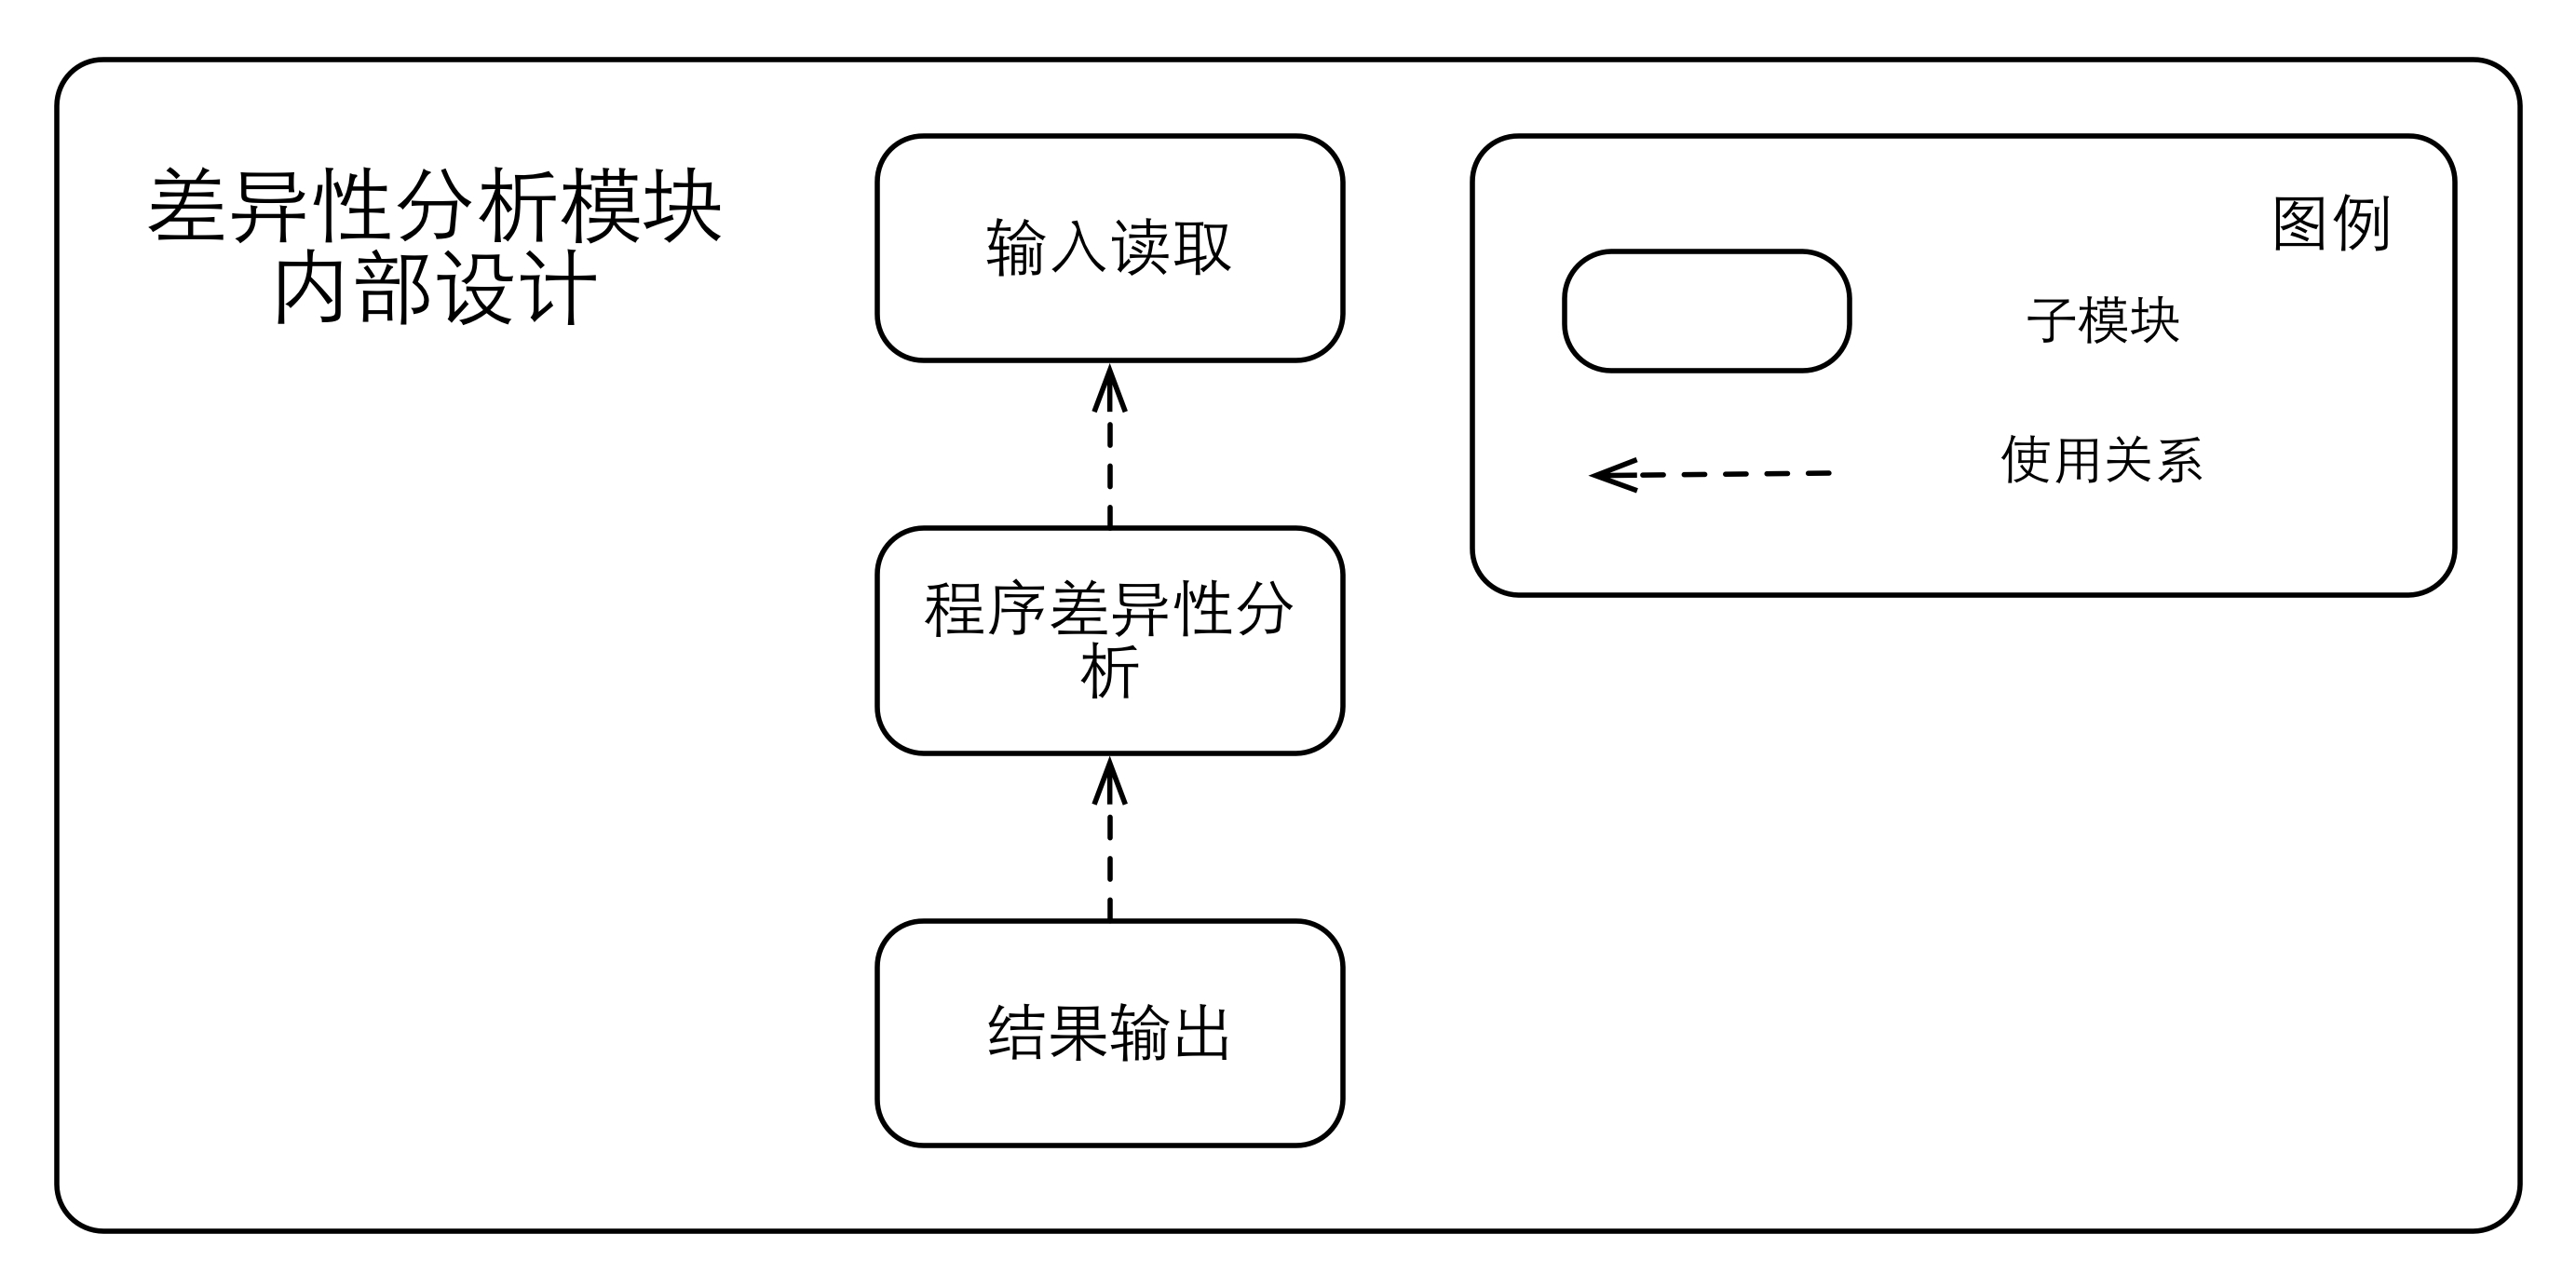
\includegraphics[width=.8\columnwidth]{chap04_diff_des}
%	\caption {模块设计}
%	\label {des_diff}	
%\end{figure}
%
%
%\begin{table}
%	\caption{输入输出对照表}
%	\label{differ_io}
%	\centering
%	\begin{tabular}{lc}
%		\toprule[1.5pt]
%		{\heiti 输入输出} & {\heiti 描述}\\\midrule[1pt]
%		$v_1$ & 源代码 \\
%		$v_2$ & 源代码 \\
%		$change\_set$ & 变更集合 \\
%		\bottomrule[1.5pt]
%	\end{tabular}
%\end{table}
%
%\subsubsection{实现}
%
%在该模块的实现过程中,采用了ASTro工具来完成具体的程序间差异分析过程。
%
%因而实际上该模块的输入输出可以参考表\ref {differ_io2}。
%
%\begin{table}[H]
%	\caption{输入输出对照表}
%	\label{differ_io2}
%	\centering
%	\begin{tabular}{llc}
%		\toprule[1.5pt]
%		{\heiti 输入输出} & {\heiti 描述} & {\heiti 格式}\\\midrule[1pt]
%		输入 & 源代码 & Java\\
%		输入 & 源代码 & Java\\
%		输出 & 影响分析模块配置文件 & JPF\\
%		输出 & 变更集合 & XML\\
%		\bottomrule[1.5pt]
%	\end{tabular}
%\end{table}

ASTro工具支持对Java代码进行比对。它会比对两个源代码文件的抽象语法树,并从中抽取出对应的不同之处,形成语法结构上的变更,并将整个变更前后的AST输出,为后续的分析过程提供了所需的变更集合。

该工具将源代码按照抽象语法树的形式进行输出,其最小节点级别为基本块,并提供了丰富的差异性信息,例如两个版本的代码间其对应节点是否发生了变更等,其输出格式为XML结构化文档。利用这些输出信息,可以从中提取出需要的程序变更集合,从而进行后续的变更语义影响分析。

在实际使用中,为了满足本文的需要,在将该工具整合进来时进行了一些改进。下面将分别进行阐述。

首先,差异性分析模块对ASTro工具的输出结果进行了一定的过滤。受限于ASTro工具的具体实现,其输出结果存在着一定的问题,主要包括:
\begin{enumerate}
	\item 对某些代码文件无法完成差异性分析。这可能是由于有的代码文件过于复杂,超出了其工具的分析能力。
	\item 对某些代码文件输出结果不准确,存在误报(False Positive)的问题。这可能是受限于工具实现中差异性分析算法的精度,导致将并没有发生变更的语法结构也认为是发生了变更,并进行了分析和输出。
\end{enumerate}

对于第一个问题,由于无法知道该工具的源代码,这里无法解决,但实验结果表明该现象只是极少数。

对于第二个问题,分析其结果可以发现其中存在着误报的情况,即某些代码行并未发生变更,然而工具却报告其发生了诸如移动、先删后增之类的伪变更。同样的,由于无法知道该工具的源代码,这里不能对其差异性分析算法进行修改。因此,在实现过程中差异性分析模块将对改为其输出结果进行专门处理,将这些误报的情况进行过滤,最后保留一个真变更子集合即可。

该过滤算法可以用算法\ref {xml}进行描述。

\begin{algorithm}
	\caption{XML结果过滤算法}
	\label{xml}
	\begin{algorithmic}[1]
		\Require $c_1 = diff(v_2, v_1), c_2 = diff(v_2,v_4)$
		\Ensure 过滤掉两个变更集合中的相同变更
		\State $del_1 \gets \varnothing$
		\State $del_2 \gets \varnothing$
		\For {$i = 0$ to $sizeof(c_1)$}
		\State $tc_1 \gets c_1[i]$
		\For {$j = 0$ to $sizeof(c_2)$}
		\State $tc_2 \gets c_2[j]$
		\If {$tc_1 == tc_2$}
		\State $del_1.add(tc_1)$
		\State $del_2.add(tc_2)$
		\EndIf	
		\EndFor
		\EndFor
		\State $c_1 \gets c_1.delete(del_1)$
		\State $c_2 \gets c_2.delete(del_2)$
	\end{algorithmic}
\end{algorithm}

这里可以归纳证明这种过滤操作的正确性。由于变更对于代码的影响是直接或间接的,对于某次变更语义影响分析的结果$s$而言,假设对于其中任意一个受影响的元素$e_k$,其中$k \subset \mathbb{N}$,其影响来源可能包括如下几种可能:
\begin{enumerate}
	\item 其影响仅来源于变更$c_1$。
	\begin{itemize}
		\item 如果$c_1$为真变更,那么删除所有伪变更对于$e_k$没有影响。
		\item 如果$c_2$为伪变更,那么删除所有伪变更会导致$e_k$从集合s中被删除,但此时$e_k$本身即为伪影响,集合$s$的正确性会得到提高。
	\end{itemize}
	\item 其影响来源于多条变更$c_1,c_2\dots,c_m$,其中$m \subset \mathbb{N}$。
	\begin{itemize}
		\item 假若所有变更均为真变更,那么删除所有伪变更对于$e_k$没有影响。
		\item 假若来源变更集合中包括某几条伪变更,那么删除所有伪变更之后,仍然存在其他真变更,这些真变更仍然会在变更语义影响分析中导致$e_k$被添加到集合$s$中,因而也不会使集合$s$的正确性下降。
		\item 假若所有变更均为伪变更,那么删除所有伪变更会导致$e_k$从集合$s$中被删除,但此时$e_k$本身即为伪影响,集合$s$的正确性会得到提高。
	\end{itemize}
\end{enumerate}

可见,本文给出的过滤算法是正确的,它不会导致后续的变更语义影响分析结果$s$的正确性降低。

其次,差异性分析模块中完成了分析过程的自动化。

在实现差异性分析模块时,该模块采用了shell脚本来完成分析过程的自动化,使该模块能够循环地调用ASTro进行分析,从而实现对整个软件系统的所有代码文件进行批量化处理。若需要修改该模块的输入信息,只需要修改脚本中对应的输入即可。在这部分工作中,脚本代码主要完成了以下任务:

\begin{itemize}
	\item 输入数据定位,包括Java源代码和编译后的Class文件等。该任务为ASTro工具提供了输入信息,即不同版本的源代码文件。
	\item 获取代码文件名,以确定本次分析的对象。该任务选择了某个具体的源代码文件作为输入。
	\item 实验数据的依赖JAR包定位。该任务是为了给出ASTro工具需要的额外输入信息,用于源代码编译过程使用。
	\item 创建输出文件目录。该任务是为了指定ASTro工具的输出存放路径。
	\item 定义ASTro的输入参数,包括输入文件位置、输出文件位置、查找路径等。该任务指定了ASTro工具运行所需的其他输入信息。
	\item 调用ASTro进行单次分析。该任务即为实际的程序间语法差异性分析过程。
\end{itemize}

其中ASTro工具的使用格式可参考如下,其具体各参数的定义参考表\ref {ASTro}。\\\\
\begin{lstlisting} [style=BashInputStyle]
ASTDiffer 3/27/2013
USAGE: java ASTDiffer -original <file>.java -modified <file>.java 
-dir <output folder>
OPTIONAL: -file <fileName> -ocp <classpath> -mcp <classpath> 
-oco <outputDir> -mco <outputDir> -cs -xml
\end{lstlisting}	

\begin{table}[H]
	\caption{ASTro参数对照表}
	\label{ASTro}
	\centering
	\begin{tabular}{llc}
		\toprule[1.5pt] 
		{\heiti 参数名} & {\heiti 描述} & {\heiti 启用}\\\midrule[1pt]
		-file & 分析目标的名字 & 是 \\
		-dir & 输出路径 & 是 \\
		-ocp & 旧版本代码的Classpath & 是\\
		-mcp & 旧版本代码的Classpath & 是\\
		-original    & 旧版本代码的位置 & 是\\
		-modified   & 新版本代码的位置 & 是\\
		-xml   & 以XML格式输出结果 & 是\\
		-cs   & 以变更脚本(Change Script)格式输出结果 & 否\\
		-heu   & 以启发式的方式进行匹配 & 是\\
		\bottomrule[1.5pt]
	\end{tabular}	
\end{table}

该模块中还利用shell脚本完成了对后续分析过程的支持,使其能够自动的、批量化的创建影响分析模块所需的配置文件。配置文件为自定义的JPF格式,通过类似键值对的方式定义了各项属性的值,其属性描述可以参考表\ref {JPF_prop}所述。

\begin{table}[H]
	\caption{JPF属性对照表}
	\label{JPF_prop}
	\centering
	\begin{tabular*}{\linewidth}{lp{10cm}}
		\toprule[1.5pt]
		{\heiti 属性名} & {\heiti 描述} \\\midrule[1pt]
		target & 分析的目标 \\
		sourcepath & 源代码路径\\
		rse.ASTResults & ASTro工具的输出文件位置\\
		rse.newClass & 新版本代码的Class文件位置\\
		rse.oldClass    & 旧版本代码的Class文件位置\\
		rse.dotFile   & jpf-regression工具的Dot格式输出文件位置\\
		\bottomrule[1.5pt]
	\end{tabular*}
\end{table}

在使用shell脚本调用ASTro工具进行分析和输出影响分析模块的配置文件时,由于需要将新版本$v_2$作为对比的基准进行分析,因此需要进行相应的配置:
%\begin{itemize}
%	\item $s_1 = impact(diff(v_2,v_1),v_2)$,求得变更集合$p_1 = diff(v_2,v_1)$对版本$v_2$的影响范围$s_1$。
%	\item $s_2 = impact(diff(v_2,v_4),v_2)$,求得变更集合$p_3 = diff(v_2,v_4)$对版本$v_2$的影响范围$s_2$。
%\end{itemize}
%实际上,也就是说:
\begin{itemize}
	\item 令结果$p_1 = diff(v_2,v_1)$,即将版本$v_2$视为“旧版本”,将版本$v_1$视为“新版本”。
	\item 令结果$p_3 = diff(v_2,v_4)$,即将版本$v_2$视为“旧版本”,将在版本$v_2$上应用补丁p后的版本$v_4$视为“新版本”。
\end{itemize}

最后,整个差异性分析模块的工作流程可以参考图\ref {sec_diff}。

\begin{figure}[H]
	\centering
	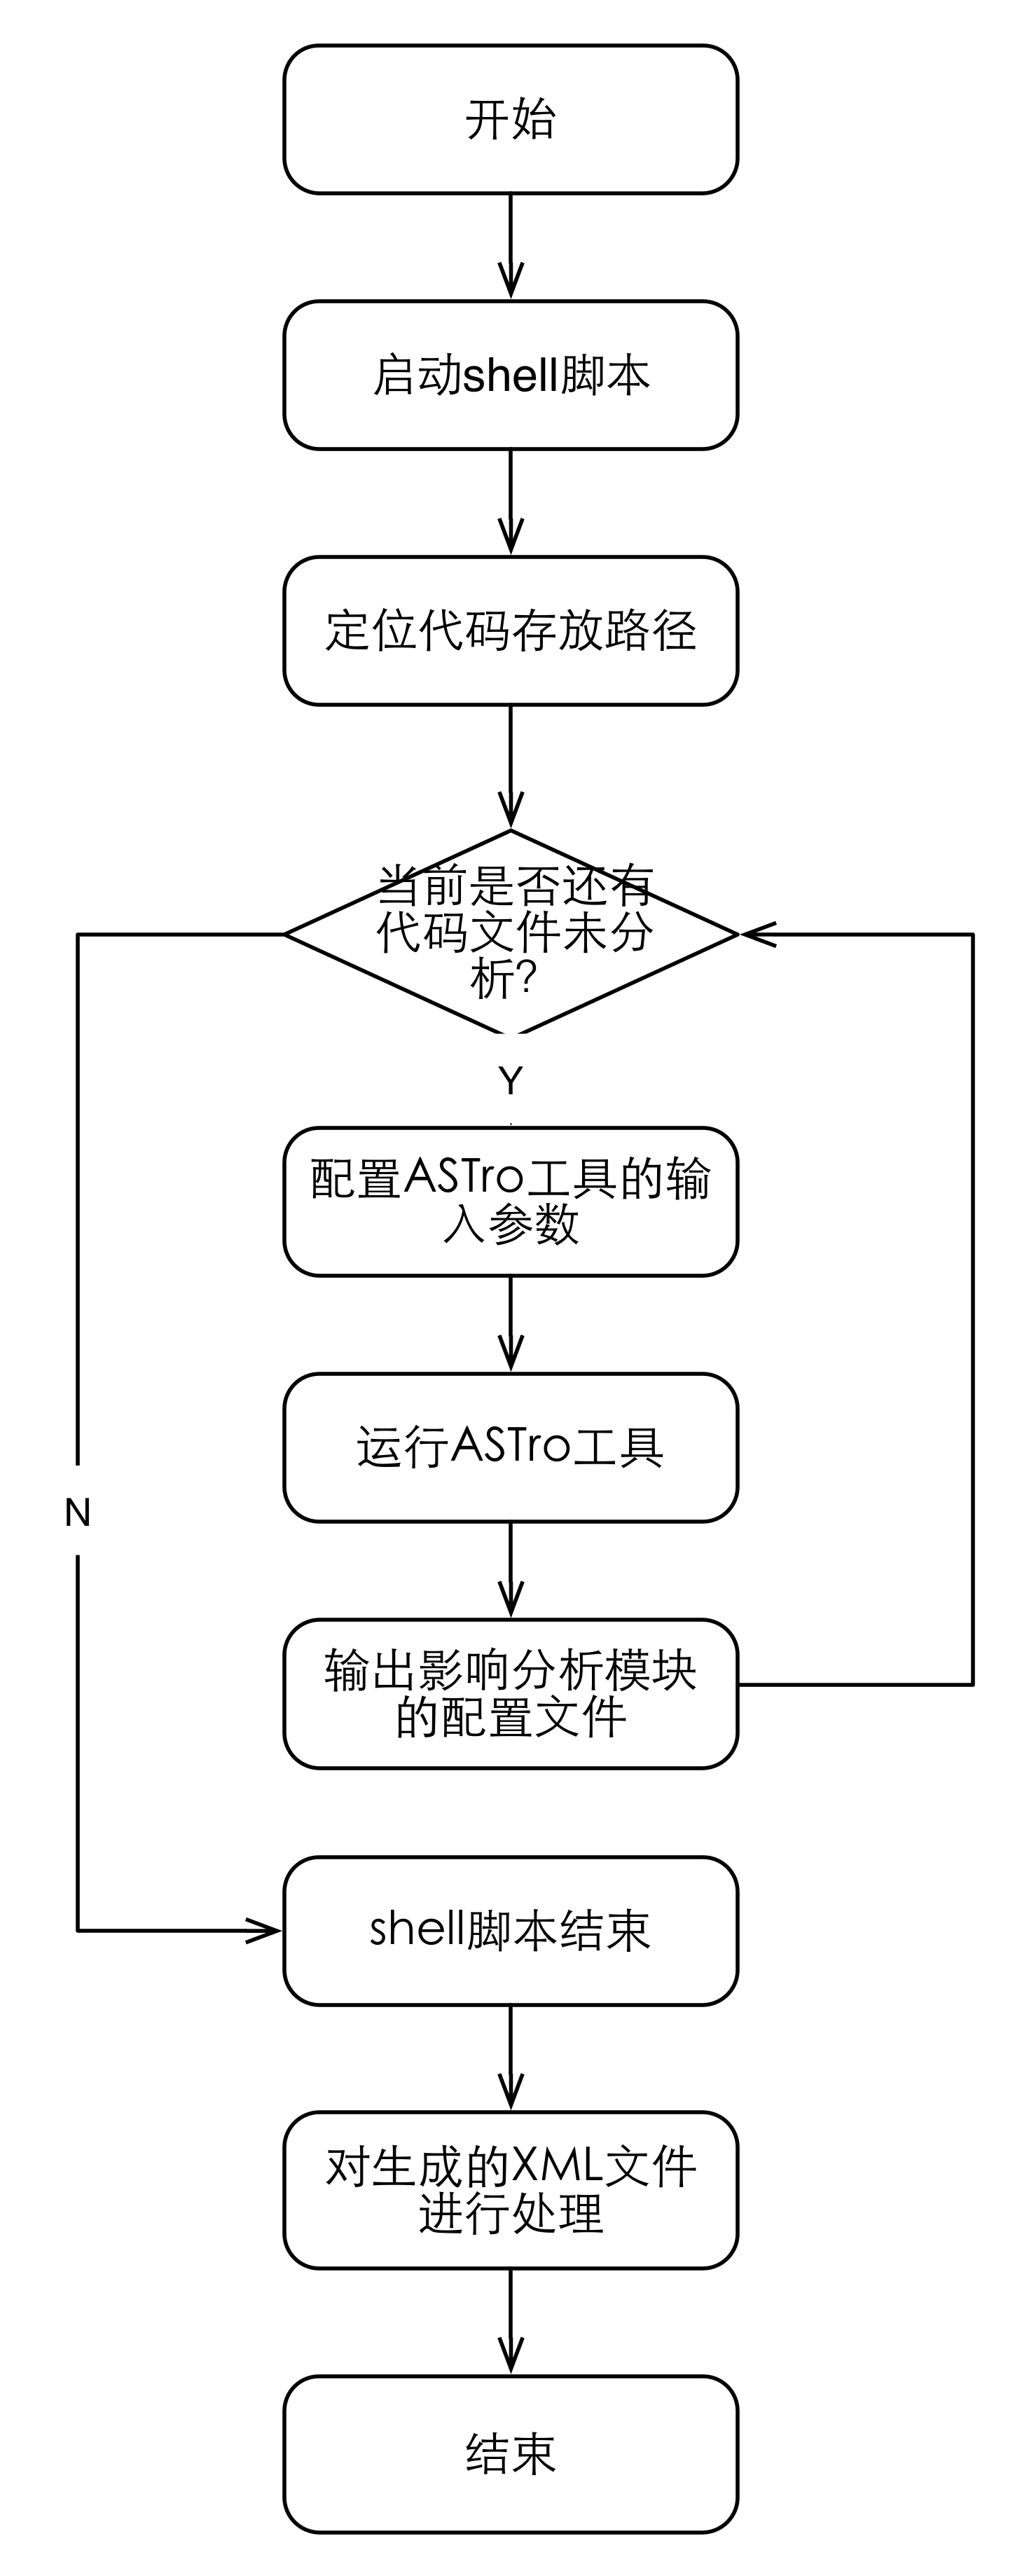
\includegraphics[height=.8\columnwidth]{chap04_differ}
	\caption {差异性分析模块流程}
	\label {sec_diff}	
\end{figure}



%图中所描述的软件变更集合可以定义如下:
%\begin{definition}
%	$ change\_set = \{ (old_i,new_i) \mid  old_i \subset Structure,new_i \subset Structure, i \subset \mathbb{N} \}$
%\end{definition}



\section{变更语义影响分析}
\label {chap_impact}
如前所述,变更语义影响分析的过程主要用于根据上一步中得到的变更集合,找到受到变更集合的语义影响的其他程序语法结构的集合,也就是所谓的变更影响域。该过程主要关注的是语法结构间存在的语义影响。
%程序变更语义影响分析是$impact$函数的具体实现,主要用于获取变更集合对其他程序结构的影响域。影响域所包含的程序结构直接或间接地受到变更集合中的元素影响。

近年来这方面也有不少比较成熟的工作,因此该模块将直接采用已有的分析工具来完成变更语义影响分析的过程。


\subsection{相关定义}

\label {sec_impact}

本节主要介绍与变更语义影响分析相关的概念和定义。以下所指的影响都是语义影响。

变更对代码的影响是由于代码之间存在的某种依赖关系而造成的,如果给出不同的依赖关系的定义,那么就会得到不同类型的影响。由此可见,影响关系即是程序代码间的耦合关系。常见的依赖关系包括控制依赖和数据依赖等。因此,影响关系可以定义如下,其中$\mathcal{S}$是某种语言的合法语法结构:

\begin{definition}
	$im: \mathcal{S} \mapsto \mathcal{S}$。该函数描述了程序语法结构之间的影响关系,$\forall s_i,s_j \subset \mathcal{S},i,j \subset \mathbb{N}$,如果$im(s_i) = s_j$,则说明语法结构$s_i$受到$s_j$的影响。其中$im(s_i) = s_j$当且仅当$s_i$依赖于$s_j$。
\end{definition}



而变更影响域,也就是变更的语义影响域是指在程序的某个限定的影响范围中,直接或间接受到变更影响的程序语法结构集合。其中影响范围描述了变更的影响传播范围。因此,变更影响域可以较形式化的定义如下,其中$\mathcal{C}$是某个版本的源代码文件中按照该语言的合法语法结构组织起来的代码,$\mathcal{P}$是变更集合:
\begin{definition}
	$impact: \mathcal{P} \times \mathcal{C} \mapsto \{\mathcal{S}\}$。$impact(p,v) = \{s_k\}$,其中$im(s_k)$要么是变更集合$p$中所改变的语法结构,要么是$impact(p,v)$中的已有元素,$p \subset \mathcal{P},v \subset \mathcal{C}, s_k \subset \mathcal{S},k \subset \mathbb{N}$。这里对$s_k$选取受限于影响范围和语法结构类型的选择。可见,变更影响域描述了变更集合在代码$\mathcal{C}$上所影响到的$\mathcal{S}$的集合。最后得到的$\mathcal{S}$的集合即为直接或间接受到变更影响的语法结构的集合,也就是所谓的变更的语义影响域(即变更影响域)。
\end{definition}

在变更影响域的计算过程中,需要考虑到其计算的精度。考虑到上文中的定义,则该过程的计算精度主要受到影响范围和语法结构类型的影响。根据前文中对于$\mathcal{S}$的定义,可以将程序中受变更影响的语法结构划分为不同的粒度,从而获得不同程度的影响\cite{petrenko2009variable},如类、方法、语句等。而影响范围的粒度则可以划分为:
\begin{enumerate}
	\item 类间:考虑变更的影响可能传播到其他类(对象)。
	\item 方法间:考虑变更的影响可能传播到其他方法内部。
	\item 方法内部:考虑变更的影响只在本方法的内部传播。
\end{enumerate}

显然,不同级别的影响范围会对变更语义影响分析的精度产生显著影响。在实践过程中,不同级别的影响范围均可采用不同的语法结构类型,以获得合适精度的变更影响域。

由此可见,$impact$函数描述了整个变更语义影响分析的过程,该分析过程需要输入代码$v$和补丁$p$,其计算结果为在$v$中某个范围内受到$p$中变更集合影响的语法结构集合,即变更影响域。

\subsection{分析方法}

在本文的兼容性检测方法中,该分析过程应当接受两个不同版本代码间的变更集合作为输入,并输出变更集合所对应的语义影响域,也就是所需的变更影响域。变更语义影响分析的过程可以通过控制流、数据流等信息分析出变更集合中每条变更对其他程序语法结构是否存在影响,并进行闭包计算以找到所有直接或间接受变更影响的语法结构。

因此,考虑到与前置的程序间语法差异性分析过程和后续的冲突检测过程进行衔接,本文要求该分析过程具备如下特征:
\begin{itemize}
	\item 接受两个不同软件版本间的变更集合和其中某个版本的代码作为输入。即该分析过程应当分析不同版本间的变更集合对于其中某个版本的影响域。
	\item 输出该变更集合所对应的影响域。即该分析过程的输出应当是变更集合对于某版本代码的影响域。
	\item 计算过程中可以指定影响范围和语法结构类型。即该分析过程可以设置分析的精度。
	\item 具有影响追踪系统,将计算影响域的过程进行记录。即该分析过程需要记录计算过程中涉及到的相关语法结构的影响关系,为后续的冲突检测过程服务,使其能根据影响关系回溯影响的来源。
\end{itemize}

%其中影响追踪系统可以定义成如下类型的函数。该函数接受一个影响域分析函数$ia(v_i,v_j)$,并返回对应的依赖关系集合。
%
%\begin{definition}
%	$impact\_track(ia(v_i,v_j)):(Code \times Code \mapsto {Structure}) \mapsto {depend}$
%\end{definition}


%该分析过程如图\ref {impact_analyzer}所述,其中的$impact$函数可以任意选择某一能够满足上述要求的变更语义影响分析算法。
%
%图中所描述的变更影响集合可以定义如下:
%\begin{definition}
%	$impact\_set = \{ (structure_i) \mid  structure_i \subset Structure, i \subset \mathbb{N}\}$
%\end{definition}
%
%\begin{figure}[H]
%	\centering
%	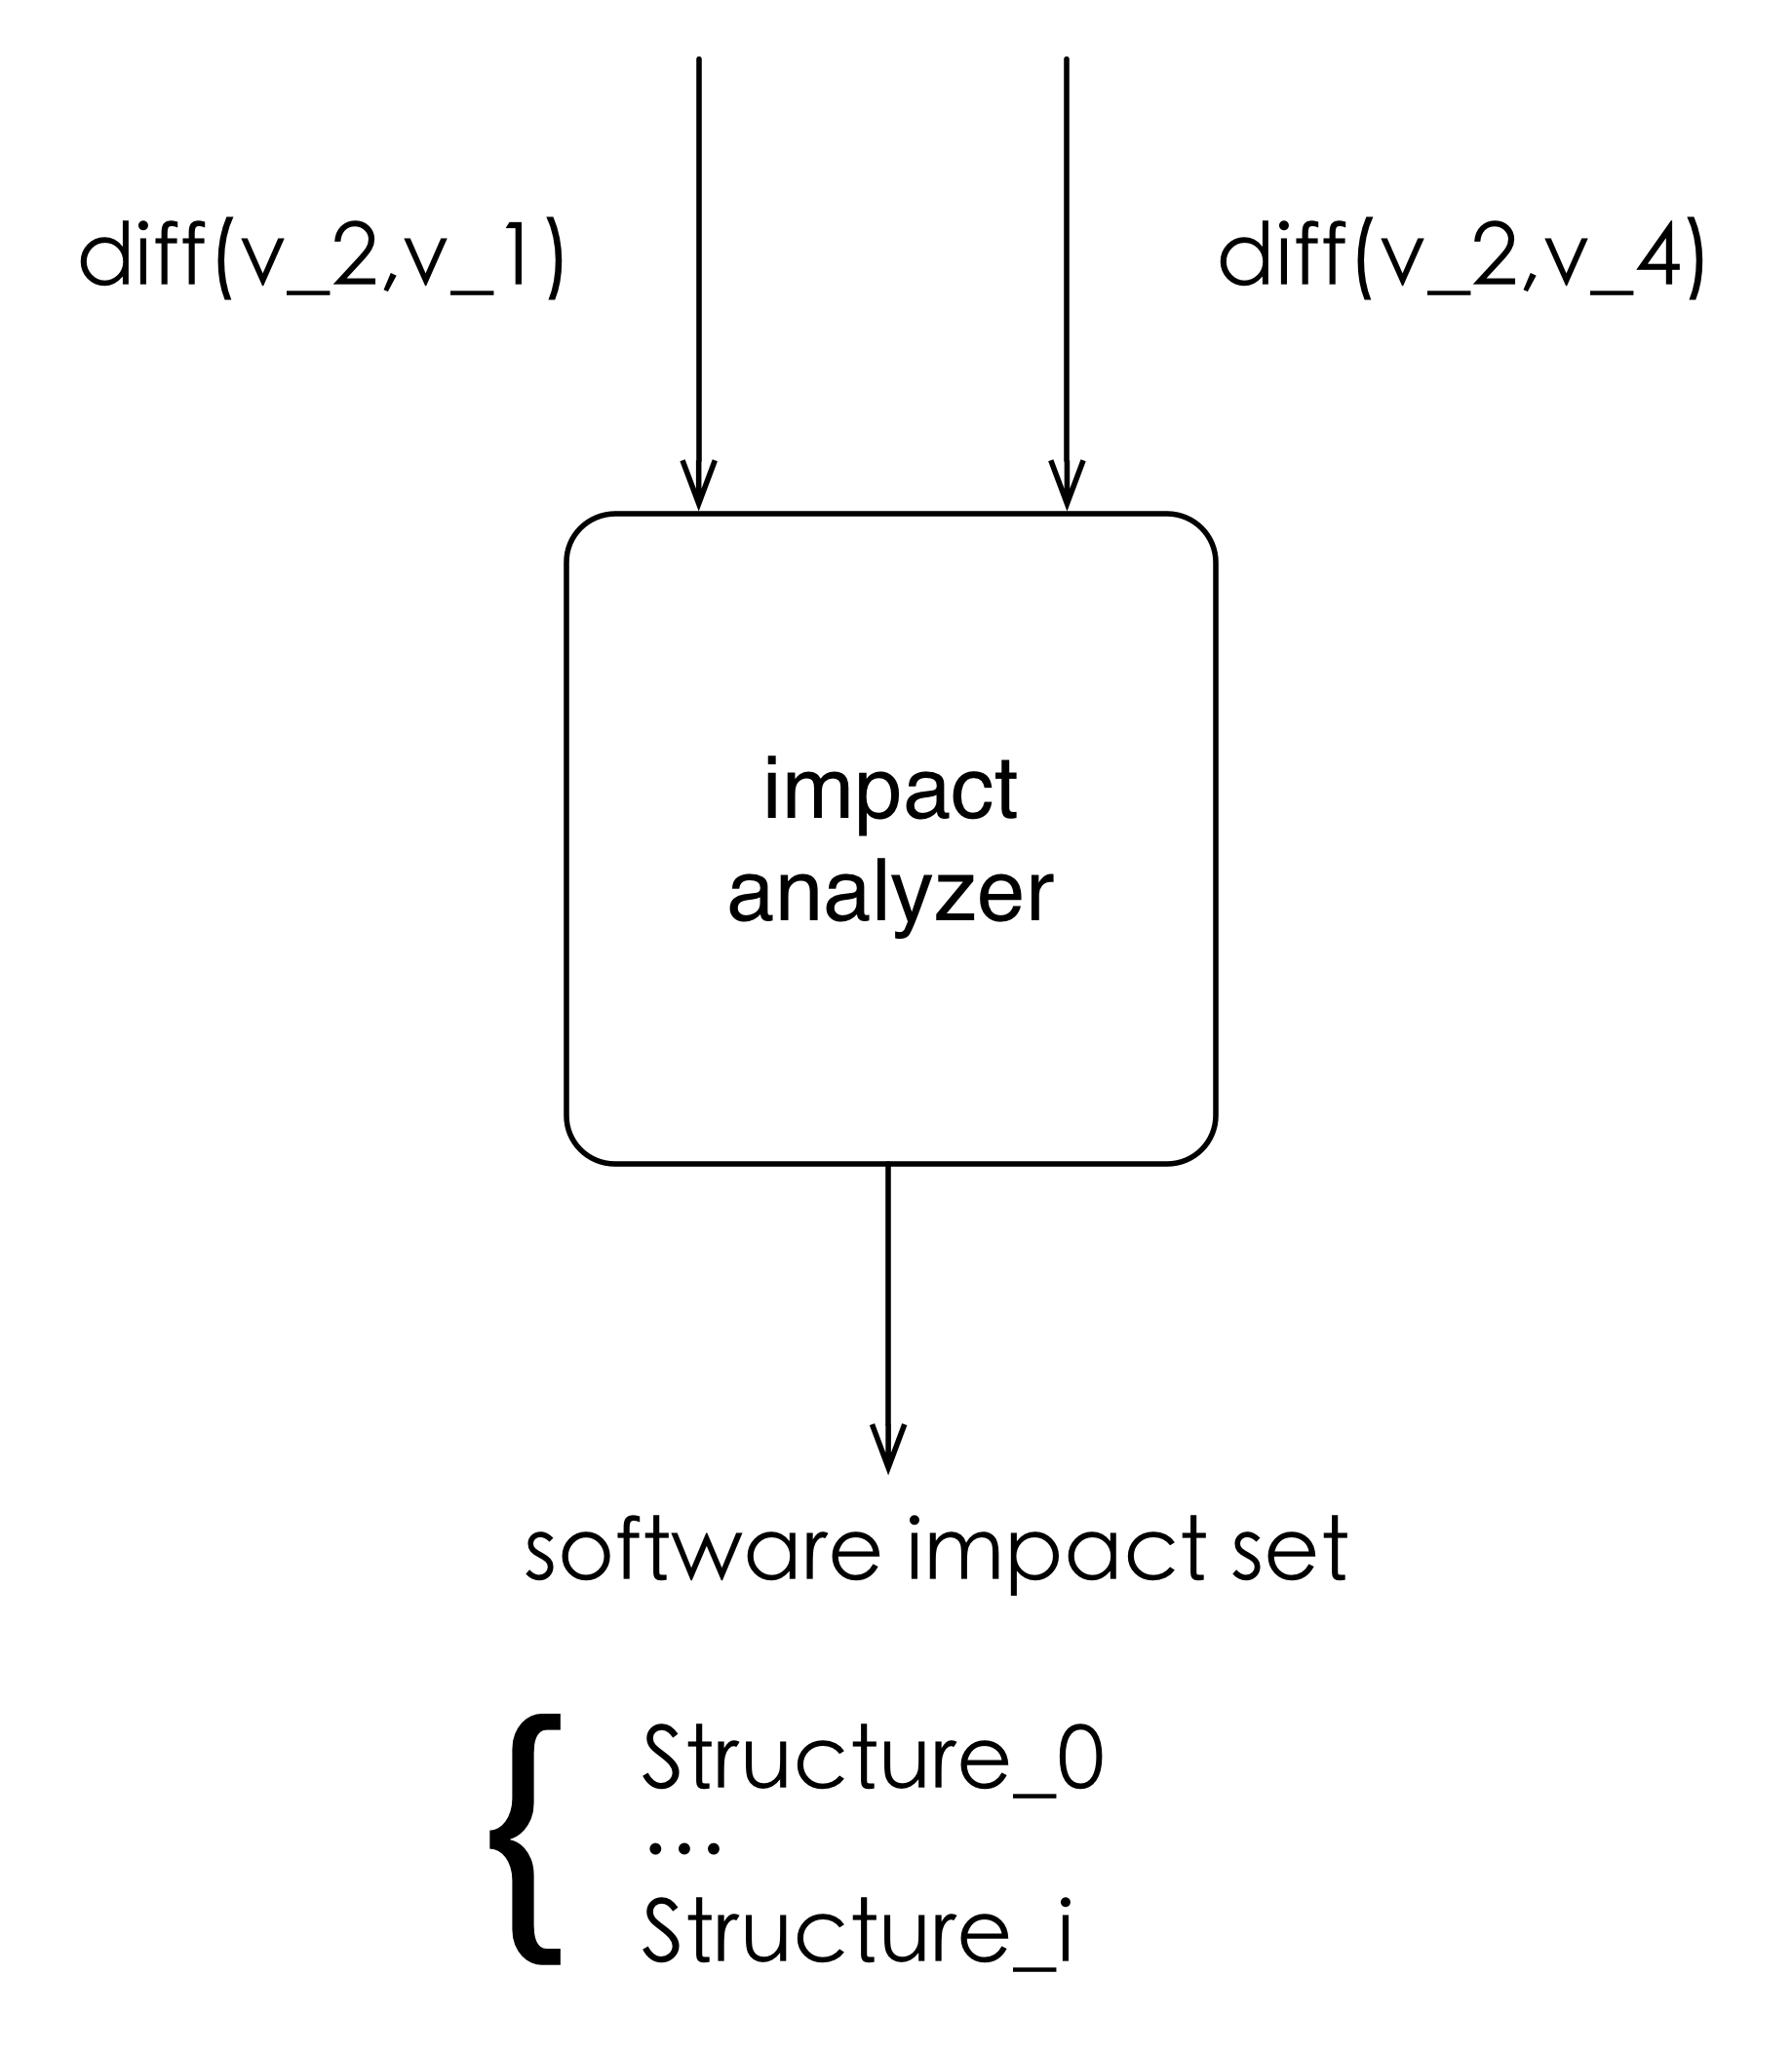
\includegraphics{chap03_impact}
%	\caption {程序间差异分析}
%	\label {impact_analyzer}	
%\end{figure}

\subsection{模块设计与实现}

在实现影响分析模块的过程中,本文主要使用了jpf-regression工具提供的变更语义影响分析算法,并选取了较为简单的分析精度设置,将影响范围限制在方法内部,将受影响的语法结构类型设置为基本块。

该子模块主要实现了$impact$函数的实际功能,它接受差异性分析模块中输出的变更集合,计算其变更影响域并将其输出。


%\subsubsection{设计}
%
%在该模块的设计中,其输入输出过程可以描述如图\ref {impact},输入输出的具体描述参见表\ref {impact_io}。
%
%考虑到该模块需要的核心任务包括:
%\begin{itemize}
%	\item 变更语义影响分析
%	\item 影响追踪:记录影响分析过程的轨迹,即影响的依赖关系$depend$。
%	\item 输入输出
%\end{itemize}
%
%因此,该模块的设计可以参考图\ref {des_impact}。
%
%该模块的流程也就可以设计成如下的形式:
%\begin{enumerate}
%	\item 读取输入
%	\item 变更语义影响分析,并进行影响追踪
%	\item 结果输出
%\end{enumerate}
%
%\begin{figure}[H]
%	\centering
%	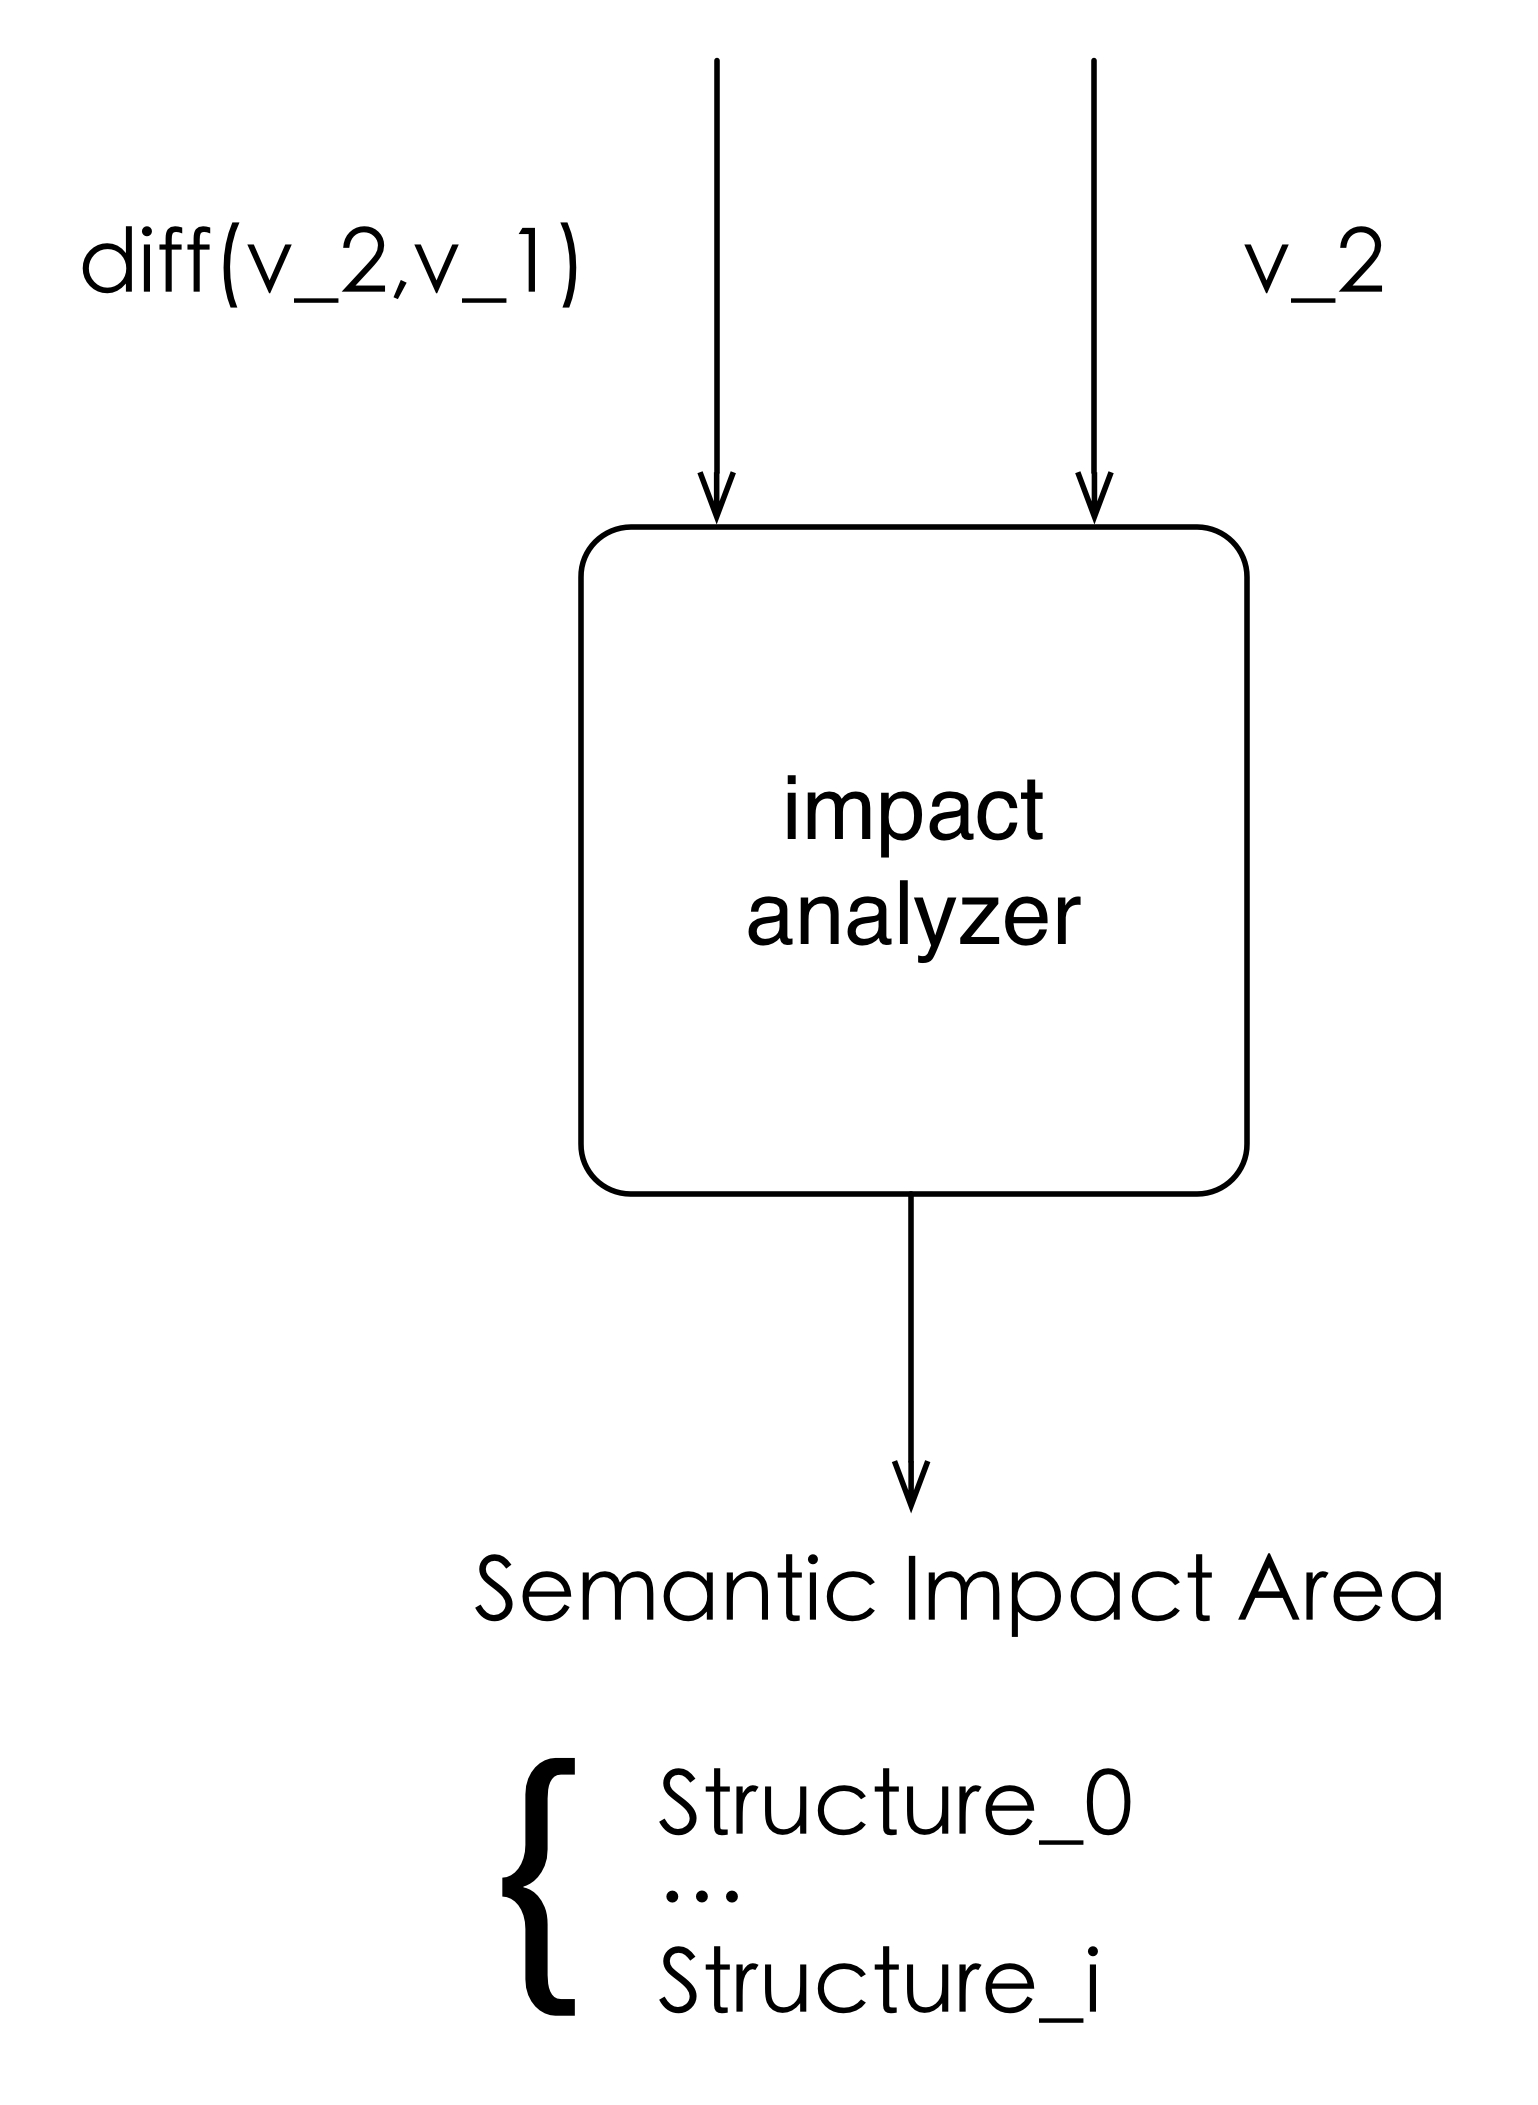
\includegraphics[height=.6\columnwidth]{chap03_impact2}
%	\caption {影响分析模块}
%	\label {impact}	
%\end{figure}
%
%
%\begin{table}[H]
%	\caption{输入输出对照表}
%	\label{impact_io}
%	\centering
%	\begin{tabular}{lc}
%		\toprule[1.5pt]
%		{\heiti 输入输出} & {\heiti 描述} \\\midrule[1pt]
%		$diff(v_2,v_1)$ & 差异性分析模块的输出,变更集合 \\
%		$v_2$ & 源代码 \\
%		语义影响域 & 语义影响域,即$v_2$中受变更影响的代码结构集合\\
%		\bottomrule[1.5pt]
%	\end{tabular}
%\end{table}
%
%\begin{figure}[H]
%	\centering
%	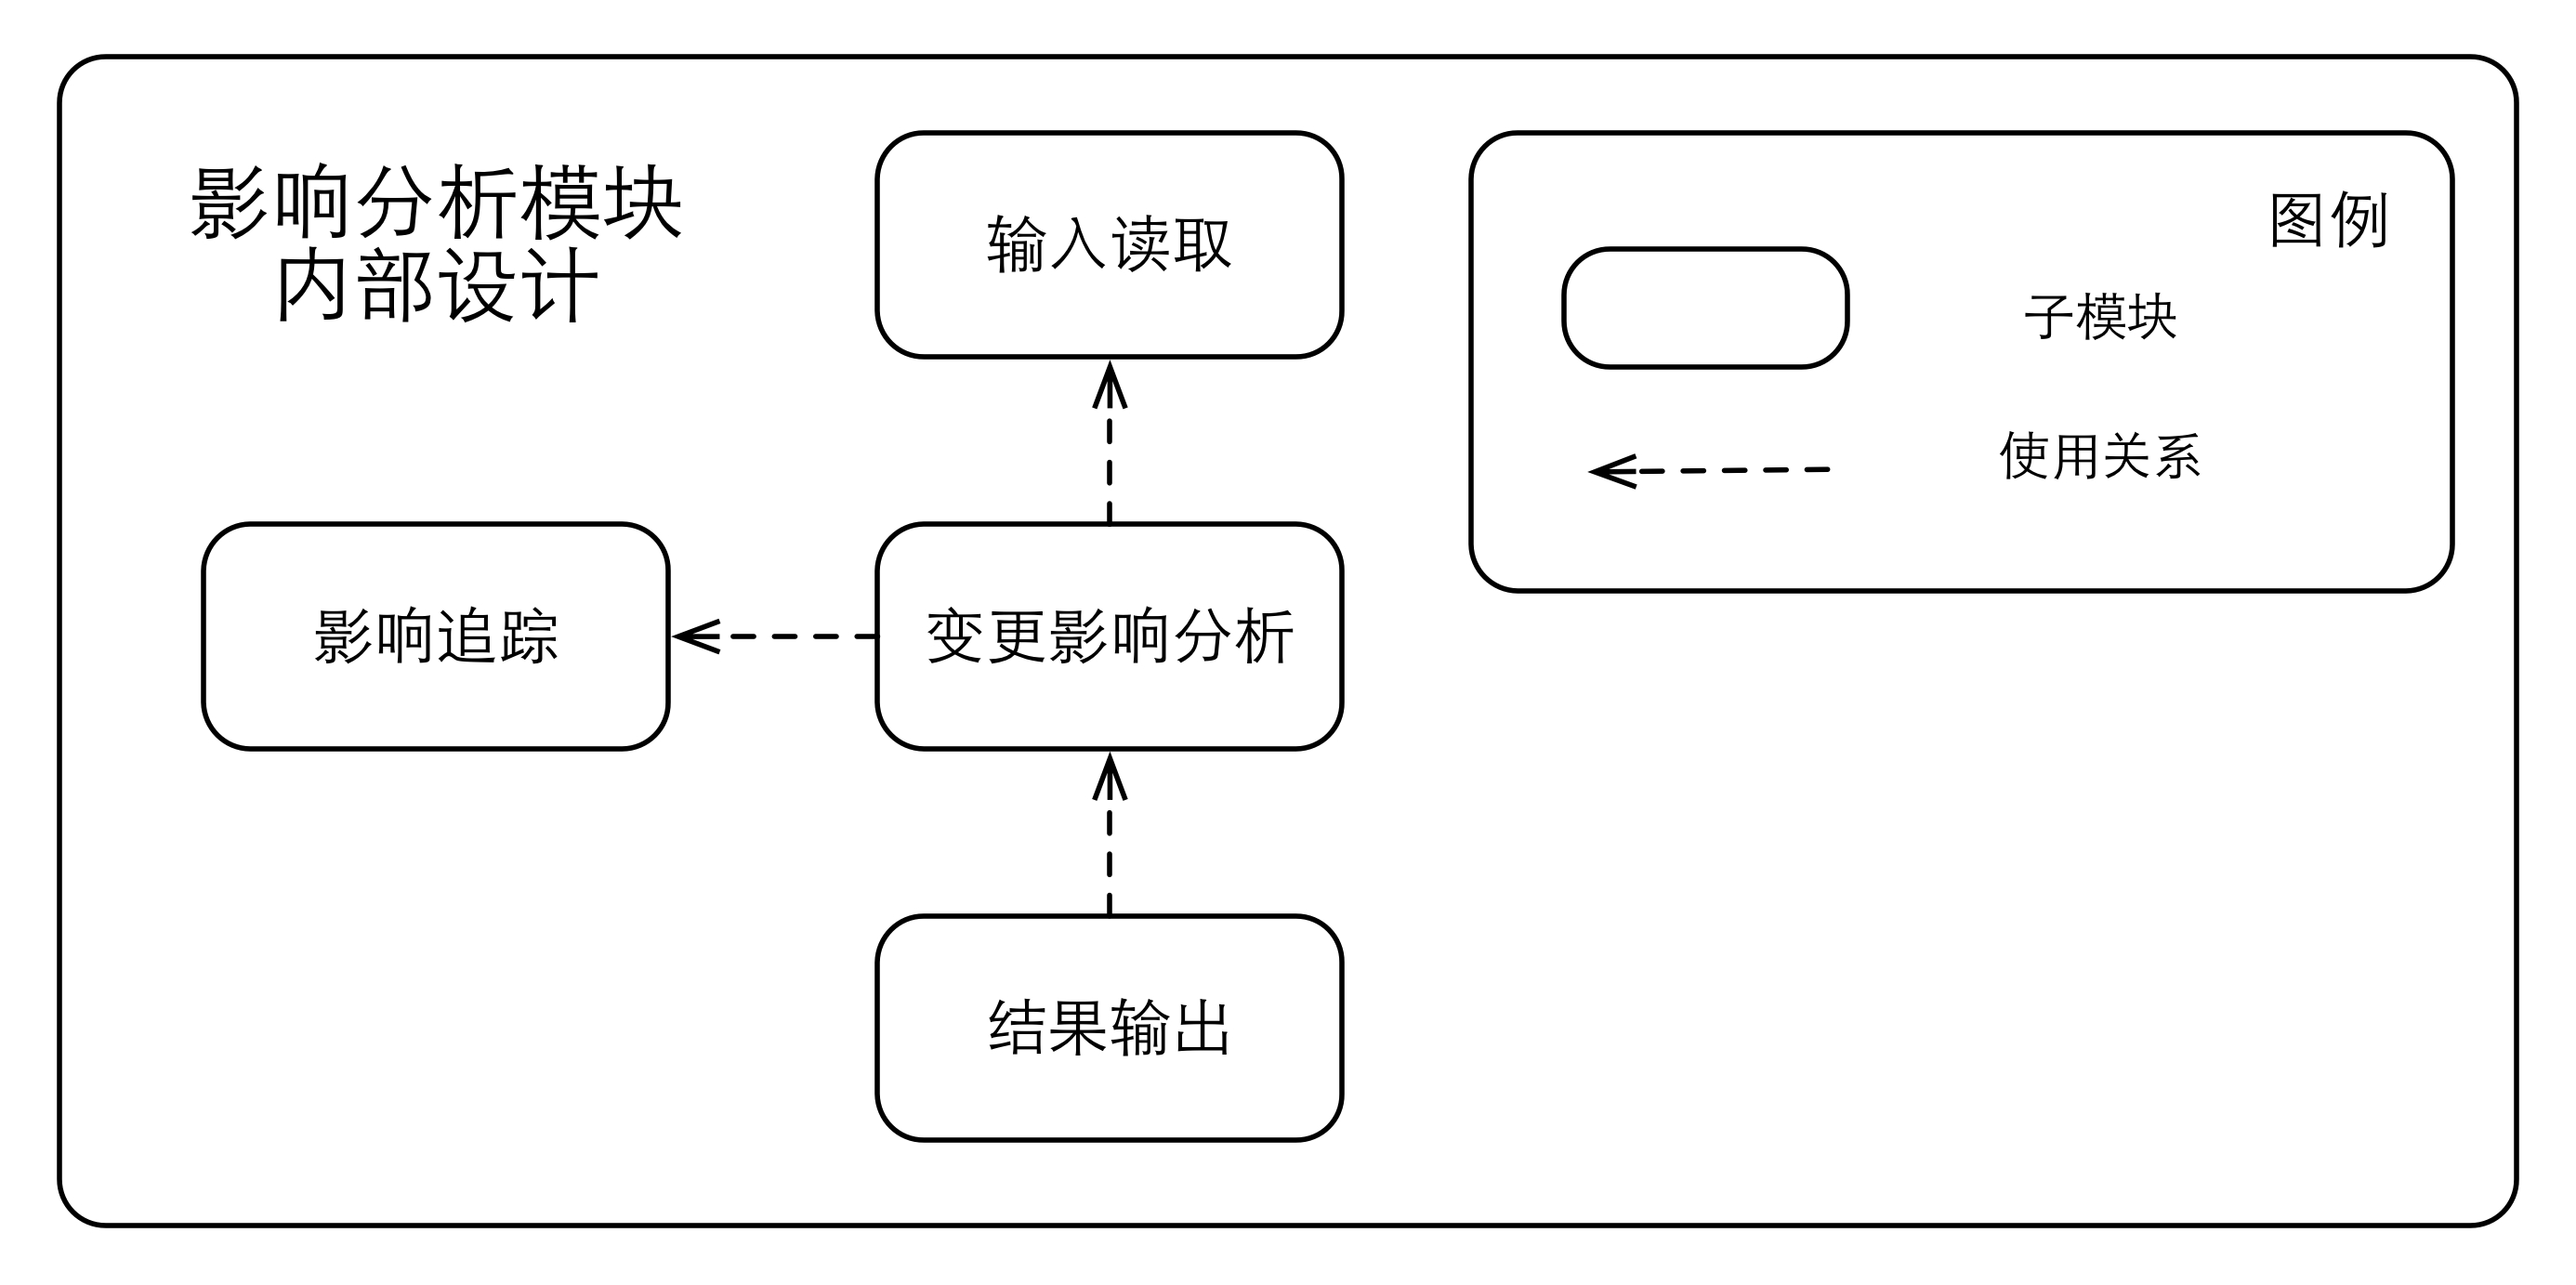
\includegraphics[width=.8\columnwidth]{chap04_impact_internal}
%	\caption {模块设计}
%	\label {des_impact}	
%\end{figure}
%
%\subsubsection{实现}

jpf-regerssion是DiSE方法在Java Path Finder软件框架下的具体实现,提供了限定在方法内的基本块级别的变更语义影响分析算法。在使用过程中,jpf-regression工具接受Java格式的源代码和ASTro提供的变更集合作为输入,并输出影响域信息至Dot文件中。

Dot是一种采用文本进行描述的图形格式,以该格式输出的实际上是整个源代码的控制流图CFG(Control Flow Graph),而变更影响域作为该控制流图承载的额外信息,在图上进行了标注。可见,该模块实际上将影响域信息输出为图形表示,其相关信息主要包括两类:
\begin{itemize}
	\item 受影响的CFG节点。这实际上就是变更影响域中的元素。可见这里受影响语法结构的级别为基本块。
	\item 节点间的影响关系。这实际上是记录了影响关系的类型,即控制依赖、数据依赖等。
\end{itemize}

%该模块的实际输入输出可以参考表\ref {impact_io2}。
%
%\begin{table}[H]
%	\caption{输入输出对照表}
%	\label{impact_io2}
%	\centering
%	\begin{tabular}{llc}
%		\toprule[1.5pt]
%		{\heiti 输入输出} & {\heiti 描述} & {\heiti 格式} \\\midrule[1pt]
%		输入 & 差异性分析模块的输出,变更集合 & XML \\
%		输入 & 源代码 & Java \\
%		输入 & 源代码 & Class \\
%		输入 & 配置文件 & JPF \\
%		输出 & 语义影响域+控制流图 & Dot \\
%		\bottomrule[1.5pt]
%	\end{tabular}
%\end{table}



然而jpf-regression工具中变更语义影响分析只是其中的一个子模块,主要用于为其后续的DiSE分析过程服务。因此影响分析模块将重用jpf-regression的代码,并对其加以改造,其主要的变化包括:
\begin{enumerate}
	\item 修改分析流程。
	\item 增加影响追踪系统。
	\item 增加错误记录系统。
	\item 使其适应大规模批量化分析的需要。
	\item 已知Bug修复。
\end{enumerate}

下面将分别进行介绍。

影响分析模块中首先对该工具的执行流程进行了修改。jpf-regression作为Java Path Finder框架的一个插件,事实上在使用时需要遵守该框架的约束,有明确的执行流程约定。然而在实践中,该流程约定并不适合于解决本文中的问题,因此本文在实现过程中对该流程进行了一定的修正。

事实上,原执行流程约定,每次分析以源代码文件中的Main函数作为入口,探索并分析Main函数所调用的其他函数。该流程对于大部分情况而言是具有实际意义的,由于只需考虑Main函数及其调用的函数,工具可以减少分析的开销并更快的得出分析结果,而忽略掉其他事实上并未被执行的函数。

然而对于本文所要解决的问题而言,该流程仅适用于部分软件系统,对于某些类型的软件系统而言可能并不适用,例如对Eclipse JDT Core项目而言,该项目主要用于为Eclipse框架下的其他组件提供服务,其功能将通过库函数的形式来提供。对于这类以库函数形式对外提供服务的源代码而言,它们既并不存在入口函数,也无法预知到底会有哪些函数会被外界所调用。由此可见,该模块应当在分析过程中覆盖其所有函数,以保证结果的完整性和正确性。

本文对于流程的修改如下所述。首先在jpf-regression工具的启动流程中去掉了图\ref {impact_process}中所示的使用JPF框架进行启动的方式,改为直接循环调用jpf-regression的核心功能,该新流程中采用RunAll类和Runjpf类来实现大规模分析的功能,其具体描述参见后文说明。其次,如图\ref {impact_process_old}所示,该模块中将待计算的方法集合由Main函数的调用函数集合更改为源代码中所有函数的集合,并在相应的影响集合计算过程中增加了影响追踪系统。

\begin{figure}[H]
	\centering
	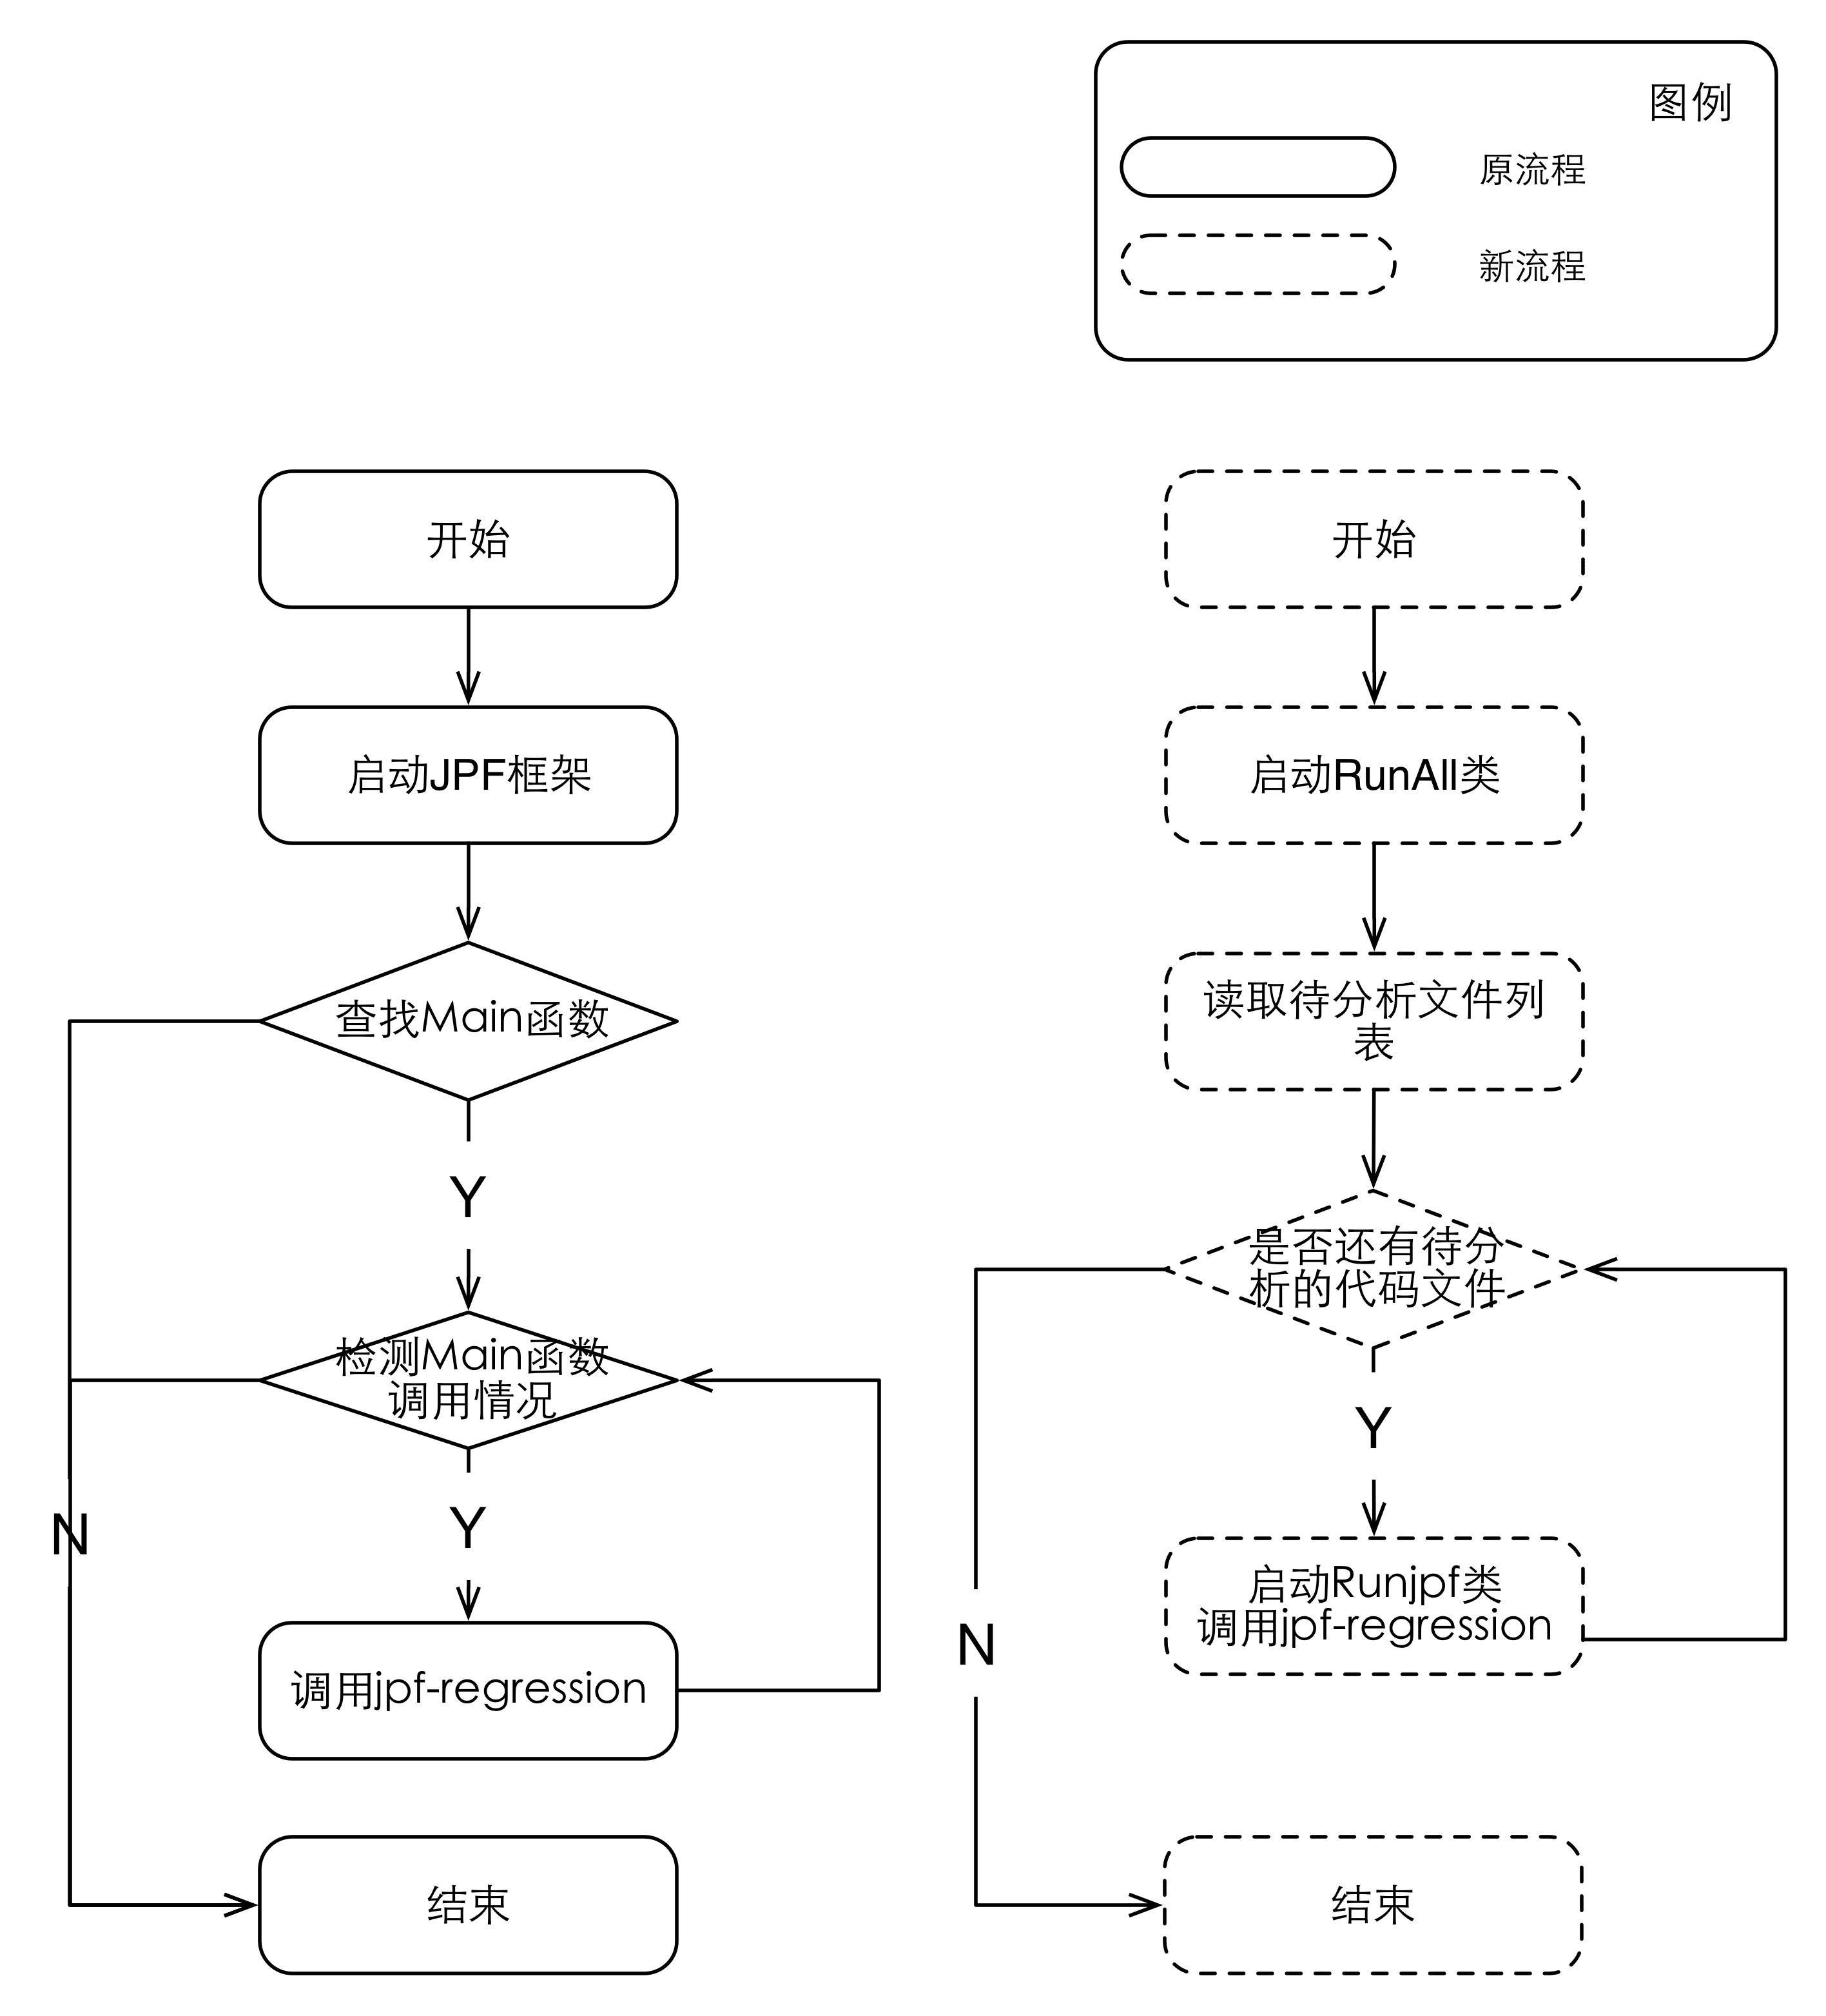
\includegraphics[height=.8\columnwidth]{chap04_jpf_launch_new}
	\caption {jpf-regression启动流程及变化}
	\label {impact_process}	
\end{figure}


\begin{figure}
	\centering
	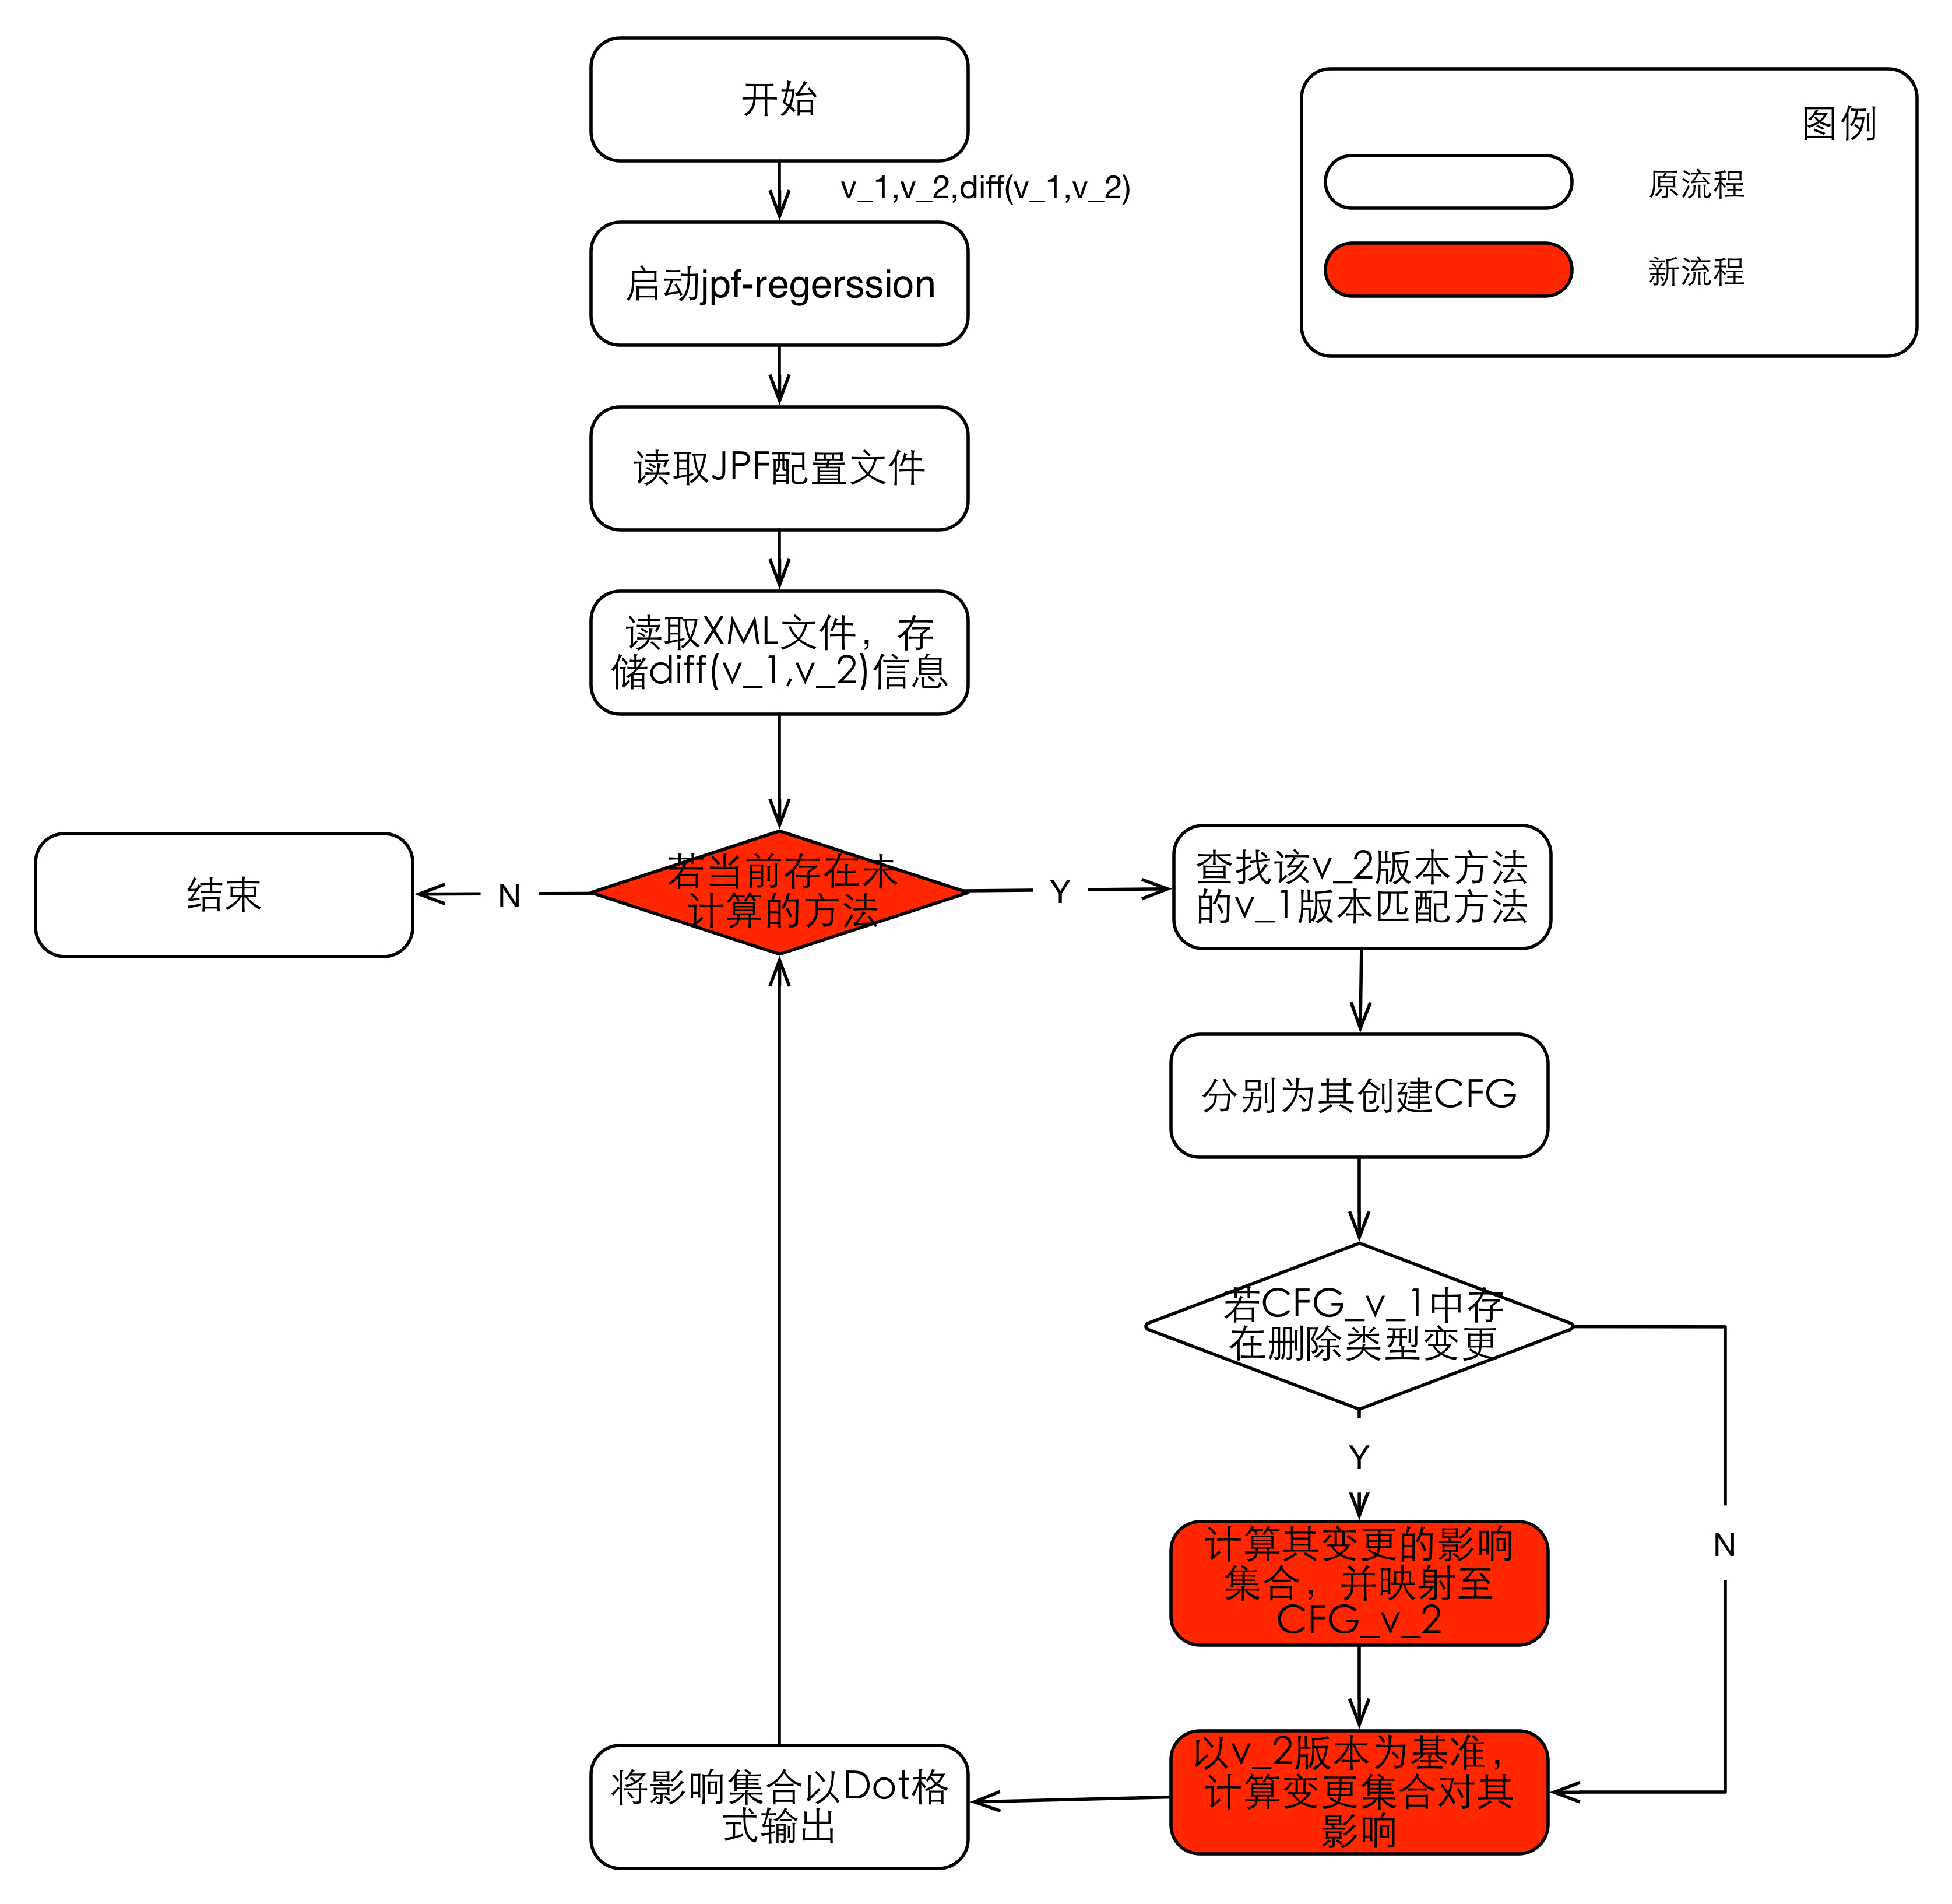
\includegraphics[width=.8\columnwidth]{chap04_jpf_old}
	\caption {jpf-regression原流程及变化}
	\label {impact_process_old}	
\end{figure}


影响分析模块中对影响追踪系统进行了实现。由于在后续的冲突判定模块中,对于找到的可能发生冲突的位置,需要输出其影响的来源以进行人工分析和判定,因此该模块将在变更语义影响分析的阶段加入影响追踪系统,以便记录下变更影响的轨迹,根据这些信息为后续的分析过程提供便利。

影响追踪系统需要存储变更影响域计算过程中找到的程序语法结构间的影响关系。由于影响的来源主要有两类,即:
\begin{itemize}
	\item 控制依赖。即某个语法结构的执行依赖于某条件语句的选择。
	\item 数据依赖。即某个语法结构中使用到了其他语法结构中定义或赋值的变量。
\end{itemize}

因此,本文实现了Dependency类族来描述该影响关系,参见图\ref {class_depend}。该类中使用了二元组depend来存储影响关系,并使用了多态机制来区分影响关系的类型。并且Dependency类族均重写了hashCode()方法和equals()方法,以便能够使用集合操作。影响追踪系统中具体使用到的数据结构可以参考表\ref {track_data}。在实现过程中,将影响关系作为控制流中承载的额外信息输出即可。

\begin{figure}[H]
	\centering
	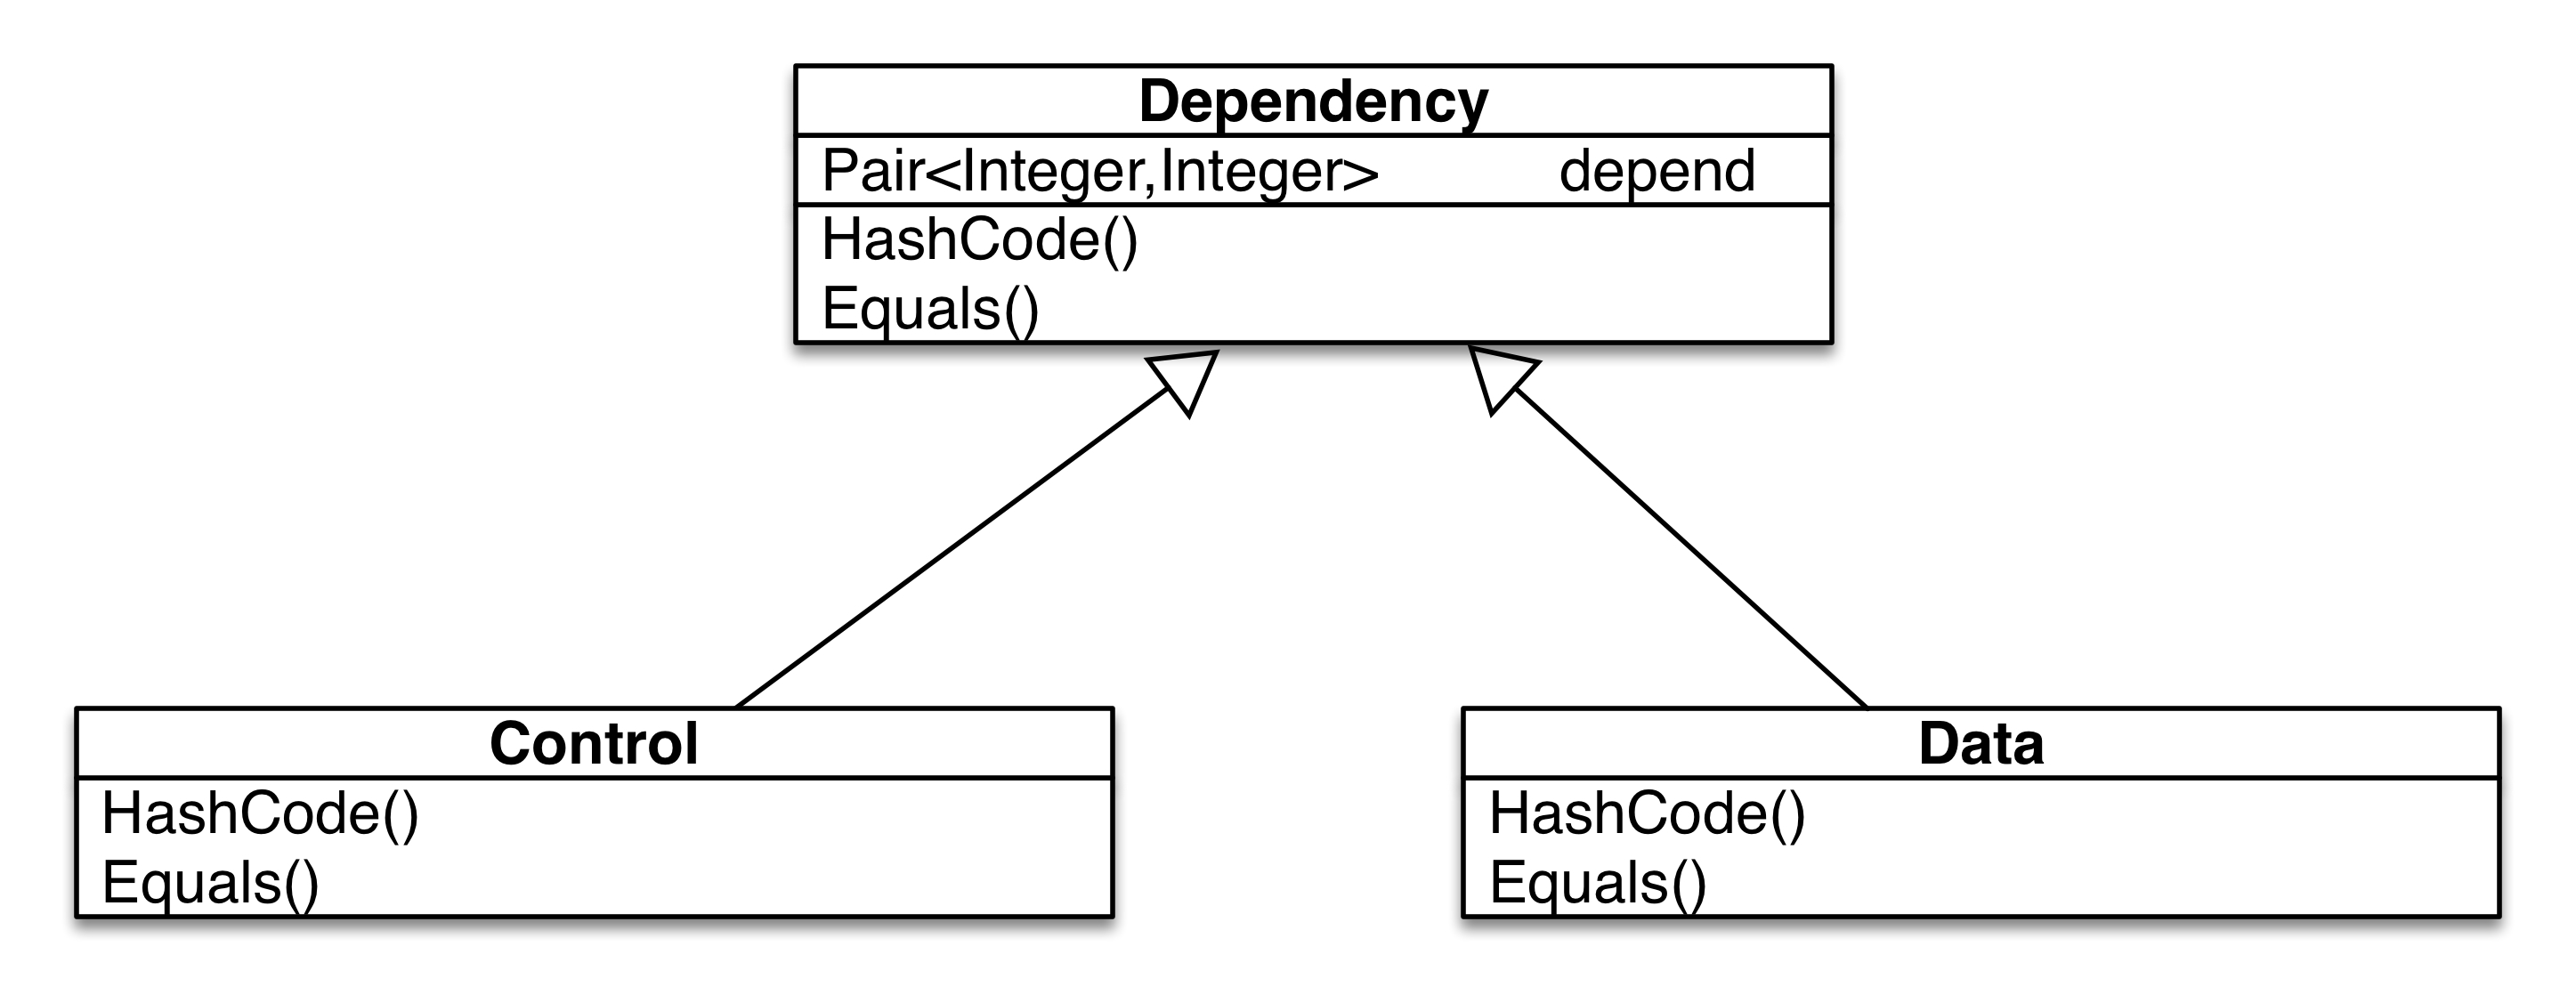
\includegraphics[width=.8\columnwidth]{chap04_depend}
	\caption {Dependency类族}
	\label {class_depend}	
\end{figure}

\begin{table}[H]
	\caption{影响关系数据结构}
	\label{track_data}
	\centering
	\begin{tabular}{lllc}
		\toprule[1.5pt]
		{\heiti 数据类型} &{\heiti 数据结构} & {\heiti 用途} \\\midrule[1pt]
		Dependency & dependency & 影响关系 \\
		Control & dependency & 控制依赖影响关系 \\
		Data & dependency & 数据依赖影响关系 \\
		Map<Integer, Set<Dependency> > & depend & 存储计算过程中的全部影响关系\\
		\bottomrule[1.5pt]
	\end{tabular}
\end{table}


影响分析模块还令分析工具适应了大规模分析过程的需要。jpf-regression工具自身只支持每次对单对源代码文件进行分析,然而考虑到软件系统在版本更新时可能有大量的源代码文件发生了变更,该模块需要具备大规模、批量化分析的能力以应对这种情况。为此,在实现过程中可以循环调用jpf-regression工具中的单次分析过程,并在上层进行封装,使大规模分析过程对于用户而言是透明的。

为了实现大规模分析过程,还需要修改工具中的某些实现细节,包括输出文件命名格式、异常处理方式等,并增加一定的数据统计能力。

在进行大规模分析的时候,工具本身自定义的输出文件命名格式需要进行修改。在原单次分析过程中,输出文件被直接命名为被分析的方法名。对于单次分析过程而言,这种设计是合适的,然而在大规模分析的情况下,由于可能存在的某些现象,例如函数重载和不同版本间的代码其方法可能无法一一匹配等,该命名方式就需要进行一定的优化。在这种情况下,可以采用一种新的命名格式:MethodName+HashCode(MethodName)+ExtensionName。

其中,MethodName为方法名,HashCode(MethodName)是利用Java语言中的hashCode方法对MethodName字符串进行计算所得到的后缀名,以保证整个文件名的唯一性。最后的ExtentionName即为文件扩展名。

大规模分析过程中还需要修改原有的异常处理模式。由于原有的jpf-regression工具只进行单次分析过程,因此一旦在运行过程中遇到问题,就会抛出异常并终止分析过程的运行。然而在实际情况中由于需要进行大规模的分析过程,如果仅仅由于单个文件的分析出错就终止整个分析过程,就会造成极大的时间和计算资源的浪费。

因此影响分析模块中修改了该工具的异常处理方式,使其在单次分析过程中如果遇到问题,只抛出异常而并不终止整个程序的运行,即采取了继续往下执行以分析其他文件的策略。然而分析中出现的异常是确实存在的,为了不丢失这类错误信息,本文为工具添加了错误记录系统,以记录每个单次分析过程中遇到的问题。

本文对程序运行过程中可能出现的报错情况进行了分类,并设计了专门的错误统计类以专门别类的对错误情况进行记录和统计。该类的实现可以参考图\ref {class_error}。其中使用到的数据结构可以参考表\ref {error_data}的说明。

\begin{figure}[H]
	\centering
	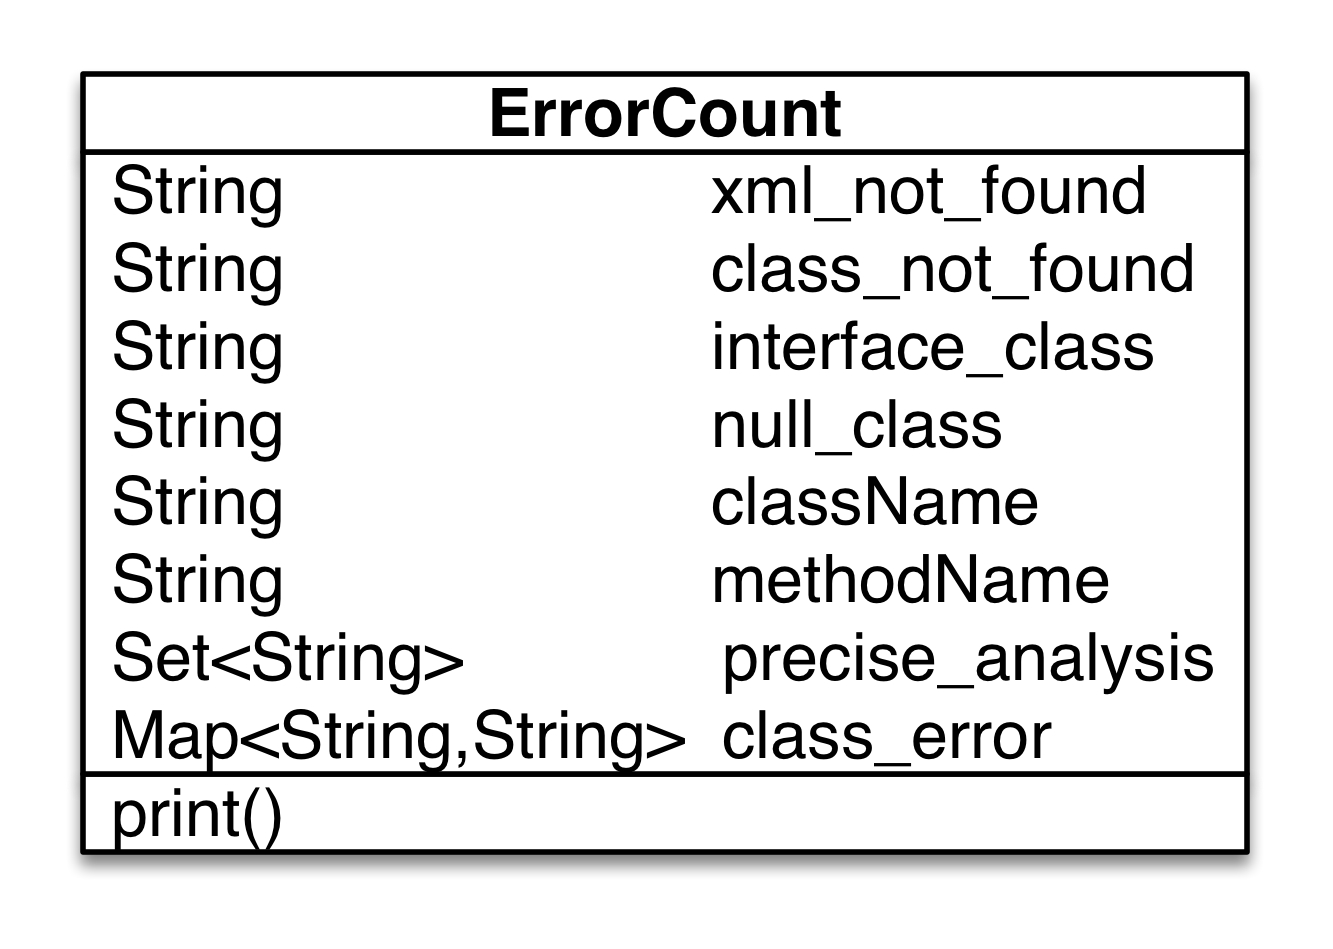
\includegraphics[height=.3\columnwidth]{chap04_error}
	\caption {ErrorCount类}
	\label {class_error}	
\end{figure}

\begin{table}
	\caption{错误记录数据结构}
	\label{error_data}
	\centering
	\begin{tabular}{lllc}
		\toprule[1.5pt]
		{\heiti 数据类型} &{\heiti 数据结构} & {\heiti 用途} \\\midrule[1pt]
		String & xml\_not\_found & 错误:XML文件未找到 \\
		String & class\_not\_found & 错误:Class文件未找到 \\
		String & interface\_class &  错误:接口类\\
		String & null\_class & 错误:类中无具体实现(如抽象类)\\
		Set<String> & precise\_analysis & 记录有多少方法在影响计算过程中出错\\
		Map<String, String> & class\_error & 记录有哪些类出现了哪些错误\\
		void & print() & 输出错误记录\\
		\bottomrule[1.5pt]
	\end{tabular}
\end{table}

大规模分析过程中,由于实验数据量非常庞大,无法像单次分析过程中那样进行人工的检查和实验结果分析。因此,影响分析模块中还增加了数据统计模块,使得程序具备一定的自动化分析实验结果的能力。

大规模分析的相关类实现可以参考图\ref {class_run_all}和图\ref {class_run_jpf}。其中涉及到的数据结构及其说明参考表\ref {run_all_data}和表\ref {run_jpf_data}。在实现中,RunAll会读取所有待分析的文件名并找到其配置文件路径,然后循环调用Runjpf对象进行单次分析过程。

\begin{figure}[H]
	\centering
	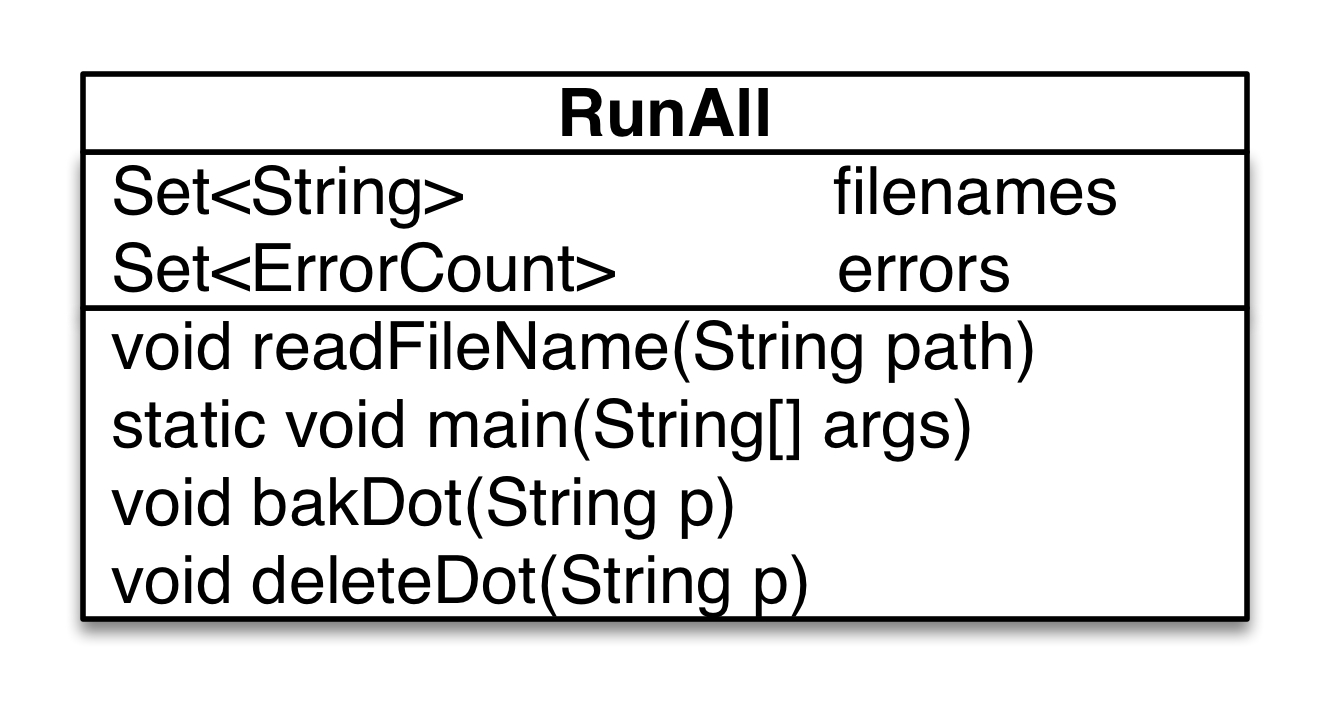
\includegraphics[width=.4\columnwidth]{chap04_run_all}
	\caption {RunAll类}
	\label {class_run_all}	
\end{figure}

\begin{figure}[H]
	\centering
	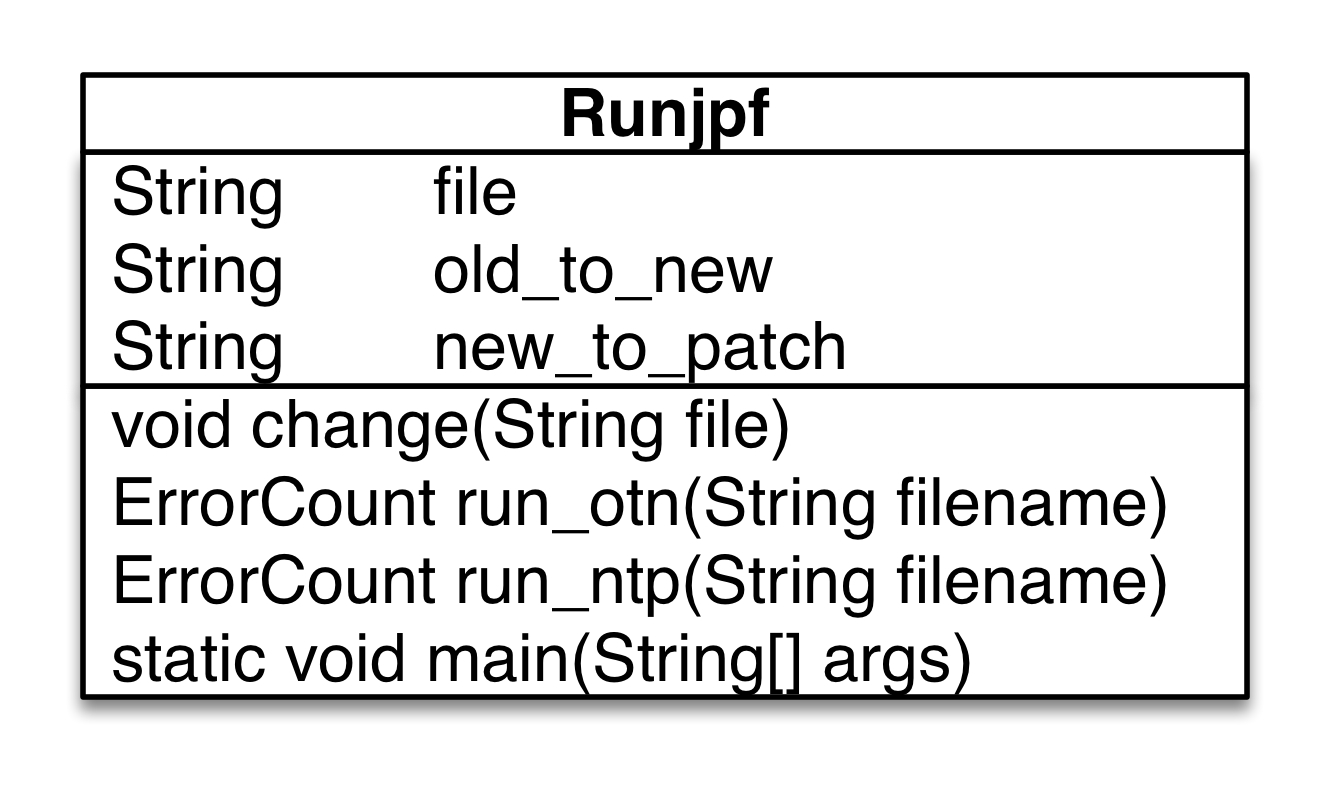
\includegraphics[width=.4\columnwidth]{chap04_run_jpf}
	\caption {Runjpf类}
	\label {class_run_jpf}	
\end{figure}

\begin{table}
	\caption{RunAll数据结构}
	\label{run_all_data}
	\centering
	\begin{tabular}{lllc}
		\toprule[1.5pt]
		{\heiti 数据类型} &{\heiti 数据结构} & {\heiti 用途} \\\midrule[1pt]
		Set<String> & filenames & 存储待分析的文件名 \\
		Set<ErrorCount> & errors & 存储每次分析中出现的错误 \\
		void & readFileName(String path) & 从文件中读取待分析的文件名\\
		static void & main(String[] args) & 实现大规模分析过程\\
		void & bakDot(String p) & 备份分析结果\\
		void & deleteDot(String p) & 删除分析结果\\
		\bottomrule[1.5pt]
	\end{tabular}
\end{table}

\begin{table}
	\caption{Runjpf数据结构}
	\label{run_jpf_data}
	\centering
	\begin{tabular}{lllc}
		\toprule[1.5pt]
		{\heiti 数据类型} &{\heiti 数据结构} & {\heiti 用途} \\\midrule[1pt]
		String & file & 待分析文件名\\
		String & old\_to\_new & $impact(diff(v_2,v_1),v_2)$过程的配置文件位置\\
		String & new\_to\_patch & $impact(diff(v_2,v_4),v_2)$过程的配置文件位置\\
		void & change(String file) & 改变当前需要读取的配置文件\\
		ErrorCount & run\_otn(String filename) & 运行$impact(diff(v_2,v_1),v_2)$过程 \\
		ErrorCount & run\_ntp(String filename) & 运行$impact(diff(v_2,v_4),v_2)$过程  \\
		static void & main(String[] args) & 实现单次分析过程\\
		\bottomrule[1.5pt]
	\end{tabular}
\end{table}


最后,影响分析模块在使用jpf-regression工具的过程中还修复了某些Bug。由于在运行过程中该工具暴露出了某些Bug,且这些Bug或多或少的导致了分析结果的正确性和精度降低,因此,在影响分析模块在实现过程中对其中某些可修复的Bug进行了修复。目前已知的Bug及其修复情况可以参见表\ref {bug_data}。
\begin{table}[H]
	\caption{Bug报告}
	\label{bug_data}
	\centering
	\begin{tabular}{lllc}
		\toprule[1.5pt]
		{\heiti Bug} &{\heiti 频率及危害} & {\heiti 修复} \\\midrule[1pt]
		内部类无法进行方法匹配 & 低,小 & 否\\
		只有单个版本代码中存在某个方法时无法进行方法匹配 & 低,小 & 是\\
		将$CFG_{v1}$的影响集合映射到$CFG_{v2}$时判断条件出错 & 高,大 & 是\\
		调用依赖JAR包jpf\_guided\_test出错 & 低,小 & 否\\
		调用依赖JAR包jpf\_symbc出错 & 低,小 & 否\\
		\bottomrule[1.5pt]
	\end{tabular}
\end{table}

\section{本章小结}

本章中主要介绍了软件变更影响域分析方法和其对应的模块设计与实现过程。
章节\ref {chap_diff}中介绍了程序间差异性分析方法和其对应的模块设计与实现。
章节\ref {chap_impact}中介绍了变更语义影响分析方法和其对应的模块设计与实现。
